\section{Combined genset and inverter}
\label{app:combined_genset_and_inverter}
\subsection*{Purpose:}
The purpose of this journal is to test how the genset react when the inverter is carrying the majority of the load. 

\subsection*{Equipment}

\begin{itemize}
	\item Genset
		\begin{itemize}
			\item \textbf{Engine:} Deutz; BF 4M 2012
			\item \textbf{Alternator:} Leroy Somer; LSA 42.3 L9 C6/4
			\item \textbf{Governor:} Deutz; EMRII("EMR2")
			\item \textbf{AVR:} DEIF; DVC310 
		\end{itemize}
		\item Inverter
		\begin{itemize}
			\item \textbf{SMA:} STP25000TL-30
			\item \textbf{DC sources:} 2 x Regatron: TopCon DC Power supply \newline (TC.P.10.1000.400.NS+1.TFE.HMI)
		\end{itemize}
		\item dSPACE unit (AAU: 61508)
		\item Hioki (datasheets are found under the path \path{CD:Hioki/}).
		\begin{itemize}
			\item HIOKI MEMORY HiCORDER 8861
			\begin{itemize}
				\item 5 x 8957 (HIGH-RESOLUTION UNIT)
			\end{itemize}
			\item \textbf{Differential probes:} 3 x Metrix MX9030-Z,
			\item \textbf{Current sensors:} 3 x HIOKI 9667 FLEXIBLE CLAMP ON SENSOR
		\end{itemize}
		\item Interface (datasheet is found under the path \path{CD:dSPACE/interface}).
\end{itemize}	


\subsection*{Procedure:}

\begin{itemize}
	%\item To setup this test either Jesper Viese Knudsen or Kjeld K. Madsen needs to attend.  
	\item The interface needs to be setup with the genset. CANbus, analog readings and frequency measurement.  
	\item The Hioki scope connected to the genset.
	\item Connect computer.
	\item Load CA7\_full\_system into simulink on the computer \path{CD:simulink/CA7/CA7_full_system}.
	\item Load build\_script into matlab \path{CD:simulink/CA7/build_script}. 
	\item Compile the build\_script.
	\item Open ControlDesk.
	\item Open project CA7 inside ControlDesk.
	\item Press 'Go Online' and 'start measuring' inside ControlDesk. 
	\item Set the needed measuring time for the Hioki scope.
	\item Turn on DC power supply for inverter.
	\item Turn on Inverter.  
	\item Start Genset.
	\item Put 10 kW load on the genset.
	\item Slowly ramp the inverter up to 10 kW. 
	\item Save the data from the Hioki scope on a USB stick or transfer the data through a LAN cable to a PC.  

\end{itemize}


\subsection*{Setup:}
\begin{figure}[H]
\centering
\includegraphics[width=0.7\textwidth]{rapport/billeder/inverter_setup_with_genset}
\caption{Setup for measurement at DEIF.}
\label{fig:inverter_setup_with_genset}
\end{figure} 


\subsection*{Measurement data:}
\begin{figure}[H]
\centering
% This file was created by matlab2tikz.
%
%The latest updates can be retrieved from
%  http://www.mathworks.com/matlabcentral/fileexchange/22022-matlab2tikz-matlab2tikz
%where you can also make suggestions and rate matlab2tikz.
%
\definecolor{mycolor1}{rgb}{0.00000,0.44700,0.74100}%
%
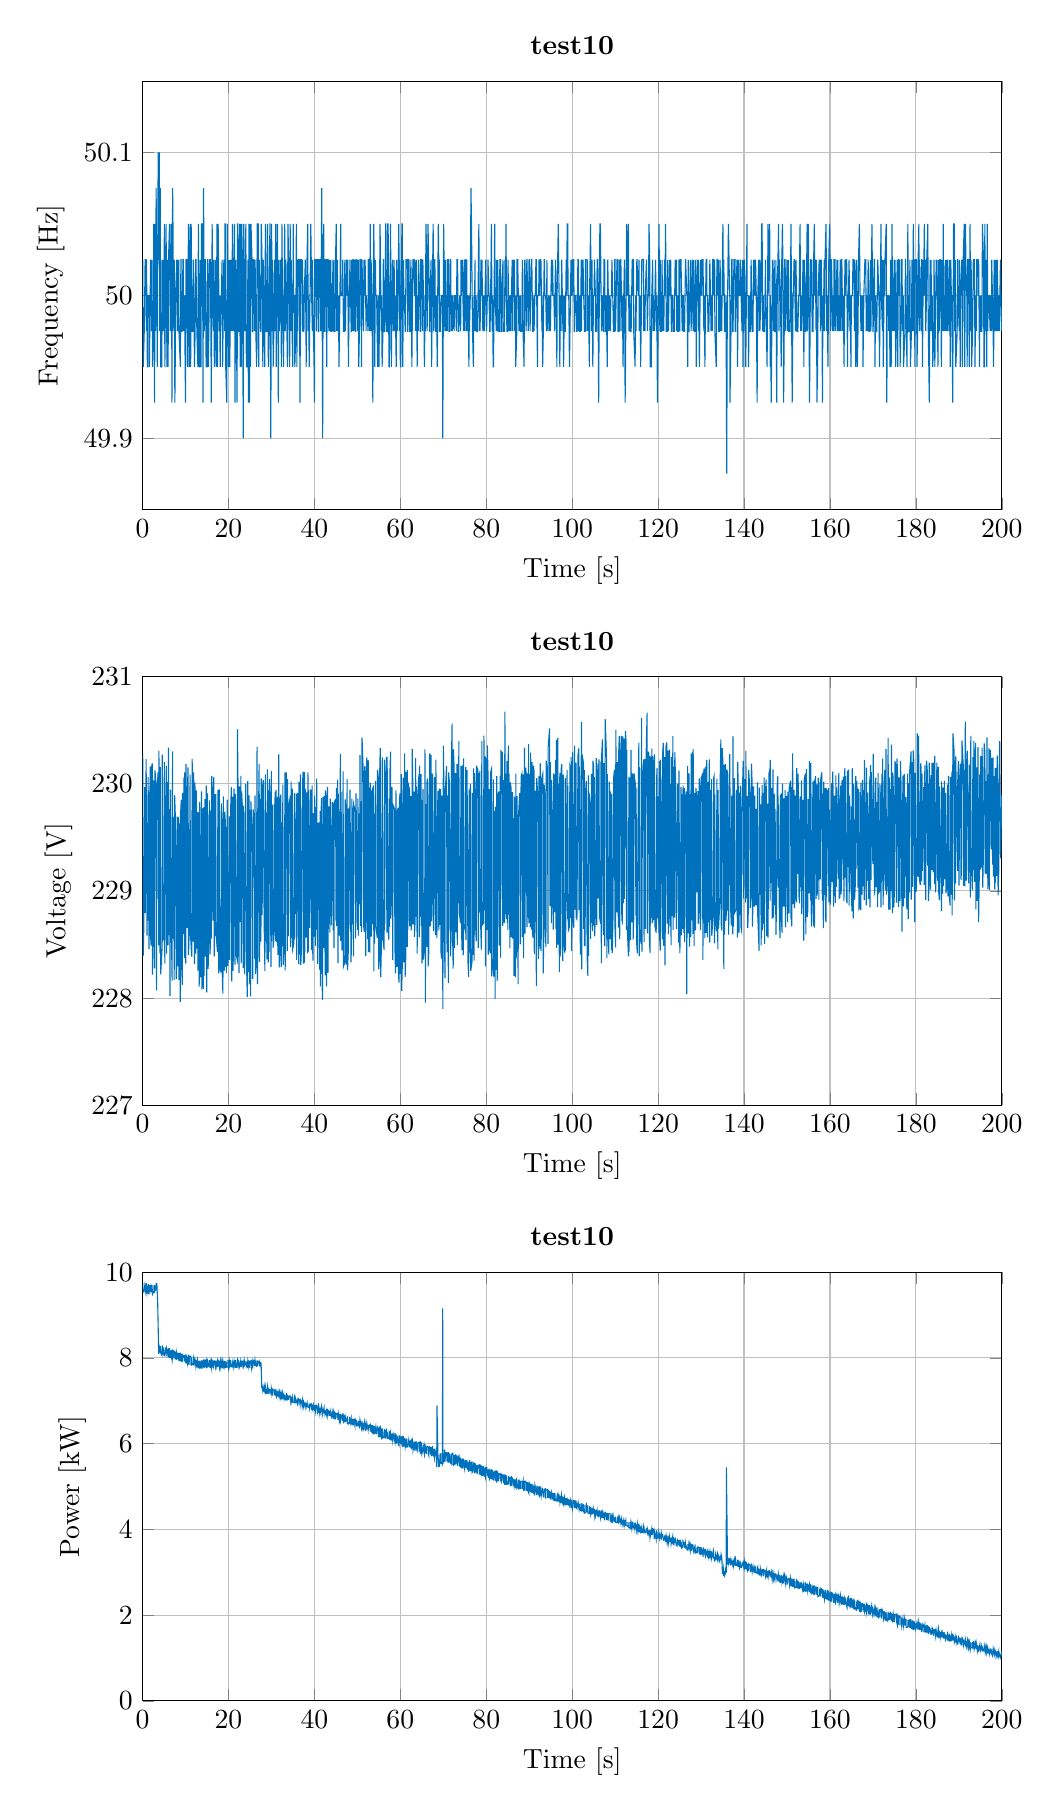
\begin{tikzpicture}

\begin{axis}[%
width=0.9\textwidth,
height=2.144in,
at={(1.297in,7.048in)},
scale only axis,
xmin=0,
xmax=200,
xlabel={Time [s]},
xmajorgrids,
ymin=49.85,
ymax=50.15,
ylabel={Frequency [Hz]},
ymajorgrids,
axis background/.style={fill=white},
title style={font=\bfseries},
title={test10}
]
\addplot [color=mycolor1,solid,forget plot]
  table[row sep=crcr]{%
0.03996	50.0250125062531\\
0.15994	49.95004995005\\
0.40004	49.9750124937531\\
0.60006	50.0250125062531\\
0.84	50.0250125062532\\
0.87998	49.9750124937531\\
0.92	50.0250125062531\\
1.11998	49.9500499500501\\
1.20002	49.9500499500499\\
1.28006	50.0000000000002\\
1.56012	50.0000000000002\\
1.60012	49.9500499500499\\
1.68016	49.9750124937532\\
1.88016	50.0250125062532\\
2.08014	49.9750124937529\\
2.20016	50.0250125062532\\
2.32014	49.9500499500501\\
2.56018	49.9750124937535\\
2.6002	50.0500500500498\\
2.8001	49.9251123315028\\
2.92018	50.0500500500503\\
3.04008	49.9750124937529\\
3.16004	50.0751126690034\\
3.43996	49.9500499500501\\
3.56004	50.0500500500503\\
3.63994	50.1002004008017\\
3.75974	50.0250125062532\\
3.87962	50.1002004008017\\
3.9995	49.9750124937535\\
4.1195	50.0751126690028\\
4.23938	49.9500499500496\\
4.4795	49.9500499500507\\
4.59954	50.0250125062532\\
4.71952	49.9750124937529\\
4.83954	50.0250125062532\\
4.95952	49.9750124937529\\
5.07954	50.0500500500503\\
5.1995	49.9500499500496\\
5.3996	50.0250125062532\\
5.4796	50.0500500500503\\
5.67958	49.9500499500496\\
5.79962	50.0250125062521\\
5.91964	49.9500499500496\\
5.99968	49.9750124937529\\
6.0397	50.0250125062532\\
6.27968	50.0500500500492\\
6.43966	49.9750124937529\\
6.67968	50.0500500500503\\
6.79962	49.9750124937529\\
6.83964	49.9251123315022\\
6.99978	50.075112669004\\
7.07968	50.0500500500503\\
7.11964	49.9750124937529\\
7.39966	50.0250125062532\\
7.51964	49.9251123315022\\
7.59972	49.9500499500507\\
7.67978	50\\
7.95978	50.0250125062532\\
8.07976	49.9750124937529\\
8.15976	50.0250125062532\\
8.27972	49.9750124937529\\
8.43976	50.0250125062532\\
8.47974	49.9750124937529\\
8.79982	49.9500499500485\\
8.91986	50.0250125062532\\
8.95984	50.0250125062532\\
9.0398	49.9750124937529\\
9.19978	49.9750124937529\\
9.39982	50.0250125062532\\
9.4798	50.0250125062532\\
9.51978	49.9750124937529\\
9.75978	50.0000000000011\\
9.99988	49.9251123315022\\
10.03994	49.9750124937529\\
10.11996	50.0250125062532\\
10.27992	50.0250125062532\\
10.47986	49.9500499500485\\
10.67986	50.0500500500514\\
10.79978	49.9750124937529\\
10.8798	49.9500499500507\\
11.0799	50.0500500500492\\
11.19986	49.9500499500507\\
11.31994	50.0500500500492\\
11.3599	50.0250125062532\\
11.43986	49.9750124937529\\
11.6799	49.9750124937529\\
11.79994	50.0250125062532\\
11.95994	50.0000000000011\\
12.07996	49.9500499500507\\
12.24002	49.9750124937529\\
12.36006	50.0250125062532\\
12.44006	50.0250125062532\\
12.64004	49.9750124937529\\
12.88004	49.9500499500507\\
13.00008	50.0500500500492\\
13.2	49.9500499500507\\
13.36012	49.9500499500485\\
13.40016	50.0250125062532\\
13.60012	49.9500499500507\\
13.72014	50.0500500500492\\
13.96016	50.0500500500492\\
14.08014	49.9251123315022\\
14.2002	50.075112669004\\
14.36008	49.9750124937529\\
14.4401	50.0250125062532\\
14.60012	50.0250125062532\\
14.80012	49.9500499500485\\
15.04022	49.9500499500485\\
15.08026	50.0250125062532\\
15.16024	50.0250125062532\\
15.28024	49.9500499500507\\
15.44028	49.9750124937529\\
15.5603	50.0250125062532\\
15.80026	50.0250125062532\\
15.96024	49.9500499500485\\
16.00028	49.9251123315066\\
16.20032	50.0500500500492\\
16.28028	50.0250125062532\\
16.48026	49.9750124937507\\
16.52028	50.0250125062532\\
16.72024	49.9500499500485\\
16.88028	49.9750124937551\\
16.9203	50.0250125062532\\
17.16026	49.9500499500485\\
17.32034	50.0500500500492\\
17.4403	49.9500499500485\\
17.60032	50.0500500500537\\
17.84024	49.9750124937507\\
17.88026	50.0000000000011\\
18.0803	49.9500499500485\\
18.12034	50.0000000000011\\
18.16034	49.9750124937507\\
18.52038	50.0250125062532\\
18.6404	49.9500499500529\\
18.92048	50.0250125062532\\
19.12048	49.9750124937507\\
19.1605	50.0500500500492\\
19.24046	50.0500500500492\\
19.3604	49.9500499500485\\
19.60046	49.9251123315022\\
19.72052	50.0500500500492\\
20.00048	49.9500499500529\\
20.12056	50.0250125062532\\
20.32056	49.9500499500485\\
20.44064	50.0250125062532\\
20.56062	49.9750124937507\\
20.60064	50.0250125062532\\
20.80058	49.9750124937507\\
20.92056	50.0500500500492\\
21.12052	49.9750124937551\\
21.32056	50.0250125062532\\
21.40054	50.0500500500537\\
21.5205	49.9251123315022\\
21.6006	49.9750124937507\\
21.72062	50.0250125062532\\
22.00064	49.9251123315022\\
22.12072	50.0500500500492\\
22.20066	50.0500500500537\\
22.24062	49.9750124937507\\
22.4406	49.9750124937507\\
22.6006	50.0500500500492\\
22.72058	49.9500499500485\\
22.84064	50.0500500500492\\
22.9606	49.9500499500529\\
23.08068	50.0500500500492\\
23.24062	50.0250125062532\\
23.44064	49.9001996007988\\
23.48072	49.9500499500485\\
23.5608	50.0500500500492\\
23.84066	49.9750124937507\\
24.04068	50.0500500500492\\
24.16062	49.9500499500485\\
24.40068	49.9500499500485\\
24.52072	50.0250125062532\\
24.6407	49.9251123315022\\
24.76076	50.0500500500492\\
24.8807	49.9251123315022\\
25.00078	50.0500500500492\\
25.1207	49.9500499500529\\
25.24076	50.0500500500492\\
25.48074	50.0250125062532\\
25.60072	49.9750124937551\\
25.68074	49.9750124937507\\
25.72076	50.0250125062532\\
25.92076	50.0250125062532\\
26.04072	49.9750124937507\\
26.20074	50.0250125062532\\
26.36072	49.9750124937507\\
26.56082	49.9500499500485\\
26.68086	50.0500500500537\\
26.92082	50.0500500500537\\
26.96078	49.9750124937507\\
27.0408	49.9500499500485\\
27.16084	50.0250125062532\\
27.2808	50.0000000000011\\
27.48084	49.9750124937507\\
27.52086	49.9750124937551\\
27.64084	50.0500500500492\\
27.80078	50.0250125062532\\
28.00076	49.9500499500485\\
28.0808	49.9999999999966\\
28.1208	50.0250125062532\\
28.44074	49.9500499500529\\
28.60076	50.0500500500492\\
28.7207	49.9750124937507\\
28.92072	49.9750124937507\\
29.08076	50.0500500500492\\
29.16072	50.0250125062532\\
29.28072	49.9500499500529\\
29.44076	49.9750124937551\\
29.64076	50.0500500500492\\
29.68072	50.0500500500492\\
29.84068	49.9001996007988\\
30.04084	50.0500500500492\\
30.16076	49.9750124937507\\
30.28076	50.0250125062532\\
30.40076	49.9500499500529\\
30.56082	49.9750124937507\\
30.76088	50.0250125062532\\
30.80086	49.9750124937507\\
31.00086	50.0500500500492\\
31.08082	50.0250125062532\\
31.1208	49.9500499500485\\
31.40092	50.0500500500492\\
31.56082	49.9750124937507\\
31.60084	49.9251123315022\\
31.72096	50.0250125062532\\
31.84092	49.9750124937507\\
32.12096	50.0250125062532\\
32.32098	49.9500499500529\\
32.441	50.0500500500492\\
32.64094	49.9750124937551\\
32.68096	50.0000000000011\\
32.80102	49.950049950044\\
33.08106	50.0500500500492\\
33.20096	49.9750124937463\\
33.361	50.0250125062532\\
33.48098	50.0000000000011\\
33.72108	49.950049950044\\
33.84114	50.0500500500492\\
34.00102	50.0250125062532\\
34.24098	49.9500499500529\\
34.36104	50.0500500500492\\
34.521	49.9750124937463\\
34.60102	50.0250125062532\\
34.80102	49.9750124937463\\
34.96106	49.9500499500529\\
35.0811	50.0500500500492\\
35.16104	50.0000000000011\\
35.361	50.0000000000011\\
35.44102	49.950049950044\\
35.6811	49.9750124937463\\
35.8011	50.0500500500492\\
35.92108	49.9500499500529\\
36.04116	50.0250125062532\\
36.16116	49.9750124937551\\
36.20118	50.0250125062532\\
36.52112	50.0250125062532\\
36.64116	49.9251123315066\\
36.72124	49.9750124937463\\
36.76126	50.0250125062532\\
37.0012	50.0250125062532\\
37.20118	49.9750124937463\\
37.2412	50.0250125062532\\
37.36118	49.9750124937551\\
37.5612	49.9750124937551\\
37.64124	50.0000000000011\\
37.88126	50.0250125062532\\
38.0412	49.9750124937551\\
38.08122	49.950049950044\\
38.28136	50.0250125062532\\
38.44128	50.0500500500492\\
38.56122	49.9750124937551\\
38.60124	50.0000000000011\\
38.8013	49.9500499500529\\
38.88134	49.9750124937463\\
39.08142	50.0250125062532\\
39.16138	50.0500500500492\\
39.36128	49.9999999999922\\
39.52128	49.9750124937551\\
39.5613	50.0250125062532\\
39.64128	50.0000000000011\\
39.92134	49.950049950044\\
40.0014	49.9251123315066\\
40.08148	50.0250125062532\\
40.28142	50.0250125062532\\
40.4814	49.9750124937463\\
40.60144	50.0250125062532\\
40.8414	50.0250125062532\\
40.92138	49.9750124937551\\
41.00142	49.9750124937551\\
41.12144	50.0250125062532\\
41.28142	50.0250125062532\\
41.4814	49.9750124937463\\
41.7213	50.0751126690106\\
41.80122	49.9999999999922\\
41.92134	49.9001996007944\\
42.0415	50.0250125062532\\
42.16144	50.0500500500492\\
42.32136	49.9750124937551\\
42.40138	49.9750124937551\\
42.4414	50.0250125062532\\
42.68144	50.0250125062532\\
42.88144	49.9500499500529\\
43.0015	50.0250125062532\\
43.1615	50.0250125062532\\
43.36148	49.9750124937463\\
43.4815	50.0250125062532\\
43.52148	49.9750124937551\\
43.68152	50.0250125062532\\
43.84146	49.9750124937551\\
44.08152	49.9750124937551\\
44.12154	50.0250125062532\\
44.24152	49.9750124937551\\
44.52156	50.0250125062532\\
44.56154	49.9750124937463\\
44.80162	49.9750124937463\\
44.92166	50.0250125062532\\
45.0816	50.0500500500492\\
45.20156	49.9750124937463\\
45.3216	50.0250125062532\\
45.52156	49.9750124937463\\
45.60158	50.0000000000011\\
45.7216	49.9500499500529\\
45.84168	49.9750124937551\\
46.12174	50.0500500500492\\
46.1617	50.0000000000011\\
46.48162	49.9999999999922\\
46.60162	50.0250125062532\\
46.6816	50.0000000000011\\
46.76162	49.9750124937463\\
46.96166	49.9750124937551\\
47.08168	50.0250125062532\\
47.20166	49.9750124937551\\
47.4817	50.0250125062532\\
47.52168	50.0000000000011\\
47.76162	50.0250125062532\\
47.92164	49.9500499500529\\
48.00168	49.9750124937463\\
48.2818	50.0250125062532\\
48.56172	49.9750124937551\\
48.60174	49.9750124937463\\
48.68178	50.0250125062532\\
48.88176	49.9750124937463\\
49.00178	50.0250125062532\\
49.1618	50.0250125062532\\
49.20178	49.9750124937463\\
49.40182	50.0250125062532\\
49.52176	49.9750124937463\\
49.64182	49.9750124937551\\
49.72186	50.0250125062532\\
49.88186	50.0250125062532\\
50.08184	49.9750124937463\\
50.20186	50.0250125062532\\
50.32184	49.9500499500529\\
50.4819	49.9750124937551\\
50.60192	50.0250125062532\\
50.8419	50.0250125062532\\
50.9619	49.950049950044\\
51.08196	50.0250125062532\\
51.44188	49.9750124937551\\
51.5219	50.0250125062532\\
51.60186	50.0000000000011\\
51.80182	50.0250125062532\\
52.04188	49.9750124937463\\
52.0819	50.0000000000011\\
52.48198	49.9750124937463\\
52.522	50.0250125062532\\
52.76198	50.0250125062532\\
52.84198	49.9750124937463\\
53.00202	50.0500500500492\\
53.122	49.9750124937463\\
53.20202	50.0250125062532\\
53.40196	50.0000000000011\\
53.60204	49.9251123315066\\
53.68212	49.9750124937551\\
53.8021	50.0500500500492\\
53.92202	50.0250125062532\\
54.042	49.9500499500529\\
54.20206	50.0250125062532\\
54.28202	50.0000000000011\\
54.48198	50.0000000000011\\
54.72202	49.950049950044\\
54.8421	50.0000000000011\\
54.96212	49.9750124937463\\
55.04216	49.9500499500529\\
55.28218	50.0500500500492\\
55.56214	49.9750124937463\\
55.64218	50.0000000000011\\
55.76222	49.950049950044\\
55.96228	49.9750124937463\\
56.0423	50.0250125062532\\
56.08228	50.0250125062532\\
56.24222	49.9750124937551\\
56.40224	49.9750124937463\\
56.60226	50.0500500500492\\
56.64222	50.0500500500492\\
56.80216	49.9750124937551\\
56.96216	49.9750124937551\\
57.08216	50.0500500500492\\
57.1621	50.0500500500492\\
57.3621	49.9500499500529\\
57.44216	49.9500499500529\\
57.7222	50.0500500500492\\
57.92216	49.9500499500529\\
57.9622	49.9750124937551\\
58.20226	50.0250125062532\\
58.24224	50.0000000000011\\
58.32224	49.9750124937551\\
58.5623	50.0250125062532\\
58.64228	49.9750124937463\\
58.80228	50.0000000000011\\
59.04232	49.9500499500529\\
59.16236	50.0250125062532\\
59.32232	49.9750124937551\\
59.5624	50.0250125062532\\
59.64236	50.0500500500492\\
59.84224	49.9750124937551\\
59.88226	50.0250125062532\\
60.00224	49.950049950044\\
60.12236	49.950049950044\\
60.36244	50.0500500500492\\
60.44238	50.0500500500492\\
60.56234	49.950049950044\\
60.76242	50.0250125062532\\
60.8024	49.9999999999922\\
60.96236	50.0000000000011\\
61.12238	49.9750124937463\\
61.2024	49.9750124937551\\
61.32246	50.0250125062532\\
61.64242	50.0250125062532\\
61.72242	49.9750124937463\\
61.76244	49.9750124937551\\
61.88248	50.0250125062532\\
62.00244	50.0250125062532\\
62.20238	49.9750124937551\\
62.40242	49.9750124937463\\
62.44244	50.0250125062532\\
62.60244	50.0000000000011\\
62.68248	49.950049950044\\
62.84258	49.9999999999922\\
62.92258	50.0250125062532\\
63.12252	50.0250125062532\\
63.3225	49.9999999999922\\
63.3625	50.0250125062532\\
63.6025	49.9750124937463\\
63.72254	50.0250125062532\\
63.92246	49.9500499500529\\
64.04254	49.9999999999922\\
64.16258	49.9750124937551\\
64.2426	50.0250125062532\\
64.48258	50.0000000000099\\
64.64258	49.9750124937551\\
64.7226	49.9750124937551\\
64.76262	50.0250125062532\\
65.00262	50.0250125062532\\
65.12258	49.9750124937551\\
65.24264	50.0250125062532\\
65.52266	49.9750124937374\\
65.6027	49.9500499500618\\
65.80278	50.0000000000099\\
65.84278	49.9750124937551\\
65.9628	50.0500500500403\\
66.16276	50.0250125062532\\
66.24272	49.9750124937551\\
66.32276	49.9999999999922\\
66.44276	50.0500500500403\\
66.60268	50.0250125062532\\
66.84268	49.9750124937374\\
66.8827	49.9750124937551\\
66.92272	50.0000000000099\\
67.16274	50.0250125062532\\
67.2827	49.950049950044\\
67.44276	49.9999999999922\\
67.64272	50.0500500500581\\
67.76268	49.9750124937551\\
67.8427	50.0250125062532\\
68.04266	50.0250125062532\\
68.16264	49.9750124937551\\
68.36274	49.9750124937374\\
68.40276	50.0000000000099\\
68.60278	49.950049950044\\
68.76286	50.0250125062532\\
68.8428	50.0500500500581\\
69.04264	49.9999999999922\\
69.08264	50.0250125062532\\
69.12262	49.9750124937551\\
69.2827	49.9750124937551\\
69.52278	50.0000000000099\\
69.80286	50.0000000000099\\
69.84286	49.9251123314889\\
69.88292	49.9001996008121\\
70.08304	50.0500500500581\\
70.36284	49.9750124937551\\
70.52288	50.0250125062532\\
70.64288	49.9750124937551\\
70.7229	50.0000000000099\\
70.92294	49.9750124937551\\
70.96296	50.0250125062532\\
71.2029	50.0250125062532\\
71.32288	49.9750124937551\\
71.44294	49.9750124937551\\
71.64296	50.0250125062532\\
71.72294	50.0250125062532\\
71.8429	49.9750124937551\\
72.00294	50.0000000000099\\
72.12294	49.9750124937551\\
72.24296	50.0000000000099\\
72.52296	49.9750124937551\\
72.643	50.0000000000099\\
72.84302	50.0000000000099\\
73.04302	49.9750124937551\\
73.12304	49.9999999999922\\
73.16304	50.0250125062532\\
73.323	50.0250125062532\\
73.48294	49.9750124937551\\
73.603	49.9750124937551\\
73.84308	50.0000000000099\\
74.04312	49.9750124937374\\
74.12314	50.0250125062532\\
74.2031	49.9999999999922\\
74.4031	50.0250125062532\\
74.56304	49.9999999999922\\
74.72302	49.9750124937551\\
74.84306	50.0250125062532\\
75.04312	49.9750124937374\\
75.16314	50.0250125062532\\
75.24312	50.0250125062532\\
75.44304	49.9750124937551\\
75.48306	50.0250125062532\\
75.52304	49.9750124937551\\
75.7631	50.0000000000099\\
75.96314	49.950049950044\\
76.04322	49.9999999999922\\
76.08322	49.9750124937551\\
76.28332	49.9999999999922\\
76.44326	50.0751126690017\\
76.56312	50.0500500500581\\
76.803	49.9750124937551\\
77.0031	49.950049950044\\
77.12316	50.0000000000099\\
77.16316	49.9750124937551\\
77.4032	50.0250125062532\\
77.44318	49.9750124937551\\
77.64316	50.0000000000099\\
77.76316	49.9750124937551\\
77.96318	49.9750124937551\\
78.08322	50.0000000000099\\
78.28322	50.0500500500581\\
78.40318	49.9750124937551\\
78.52322	50.0000000000099\\
78.56322	49.9750124937374\\
78.76326	50.0250125062532\\
78.80324	49.9999999999922\\
79.00322	50.0250125062532\\
79.20322	49.9750124937374\\
79.24324	50.0000000000099\\
79.36324	49.9750124937551\\
79.52326	49.9999999999922\\
79.56326	49.9750124937551\\
79.88342	50.0250125062532\\
80.08332	49.9750124937374\\
80.2434	50.0000000000099\\
80.36342	49.9999999999922\\
80.40342	50.0250125062532\\
80.64334	50.0000000000099\\
80.80334	49.9750124937551\\
80.88338	49.9750124937551\\
81.1234	50.0250125062532\\
81.20336	50.0500500500403\\
81.36328	49.9750124937551\\
81.4833	50.0000000000099\\
81.60332	49.9500499500618\\
81.68338	49.9500499500618\\
81.96344	50.0500500500403\\
82.08338	49.9999999999922\\
82.32338	49.9750124937374\\
82.44342	50.0250125062532\\
82.5634	49.9750124937374\\
82.68342	50.0250125062532\\
82.76342	50.0000000000099\\
82.80342	49.9750124937551\\
83.0835	49.9750124937374\\
83.16352	50.0250125062532\\
83.32348	50.0250125062532\\
83.48344	49.9750124937551\\
83.56346	49.9750124937551\\
83.64348	50.0000000000099\\
83.88348	50.0250125062532\\
83.92346	49.9750124937551\\
84.24348	49.9750124937551\\
84.36352	50.0250125062532\\
84.48348	49.9999999999922\\
84.60346	50.0500500500581\\
84.68342	50.0000000000099\\
84.80342	49.9750124937551\\
84.96344	49.9750124937551\\
85.08348	50.0250125062532\\
85.20348	49.9750124937551\\
85.2435	50.0000000000099\\
85.44352	49.9750124937551\\
85.52354	50.0000000000099\\
85.76354	49.9750124937551\\
85.84356	50.0000000000099\\
86.0436	50.0250125062532\\
86.16358	49.9750124937551\\
86.2836	50.0250125062532\\
86.40354	49.9999999999922\\
86.52352	50.0250125062532\\
86.64346	49.9750124937551\\
86.80346	49.9999999999922\\
86.84346	49.950049950044\\
87.12364	49.9750124937551\\
87.16366	50.0250125062532\\
87.3236	50.0250125062532\\
87.60354	49.9750124937551\\
87.64356	50.0000000000099\\
87.68356	49.9750124937374\\
87.96364	50.0000000000099\\
88.00364	49.9750124937551\\
88.32368	49.9750124937551\\
88.4037	50.0250125062532\\
88.56368	49.9750124937551\\
88.80376	49.9500499500618\\
88.92382	50.0250125062532\\
88.9638	49.9999999999922\\
89.0038	50.0250125062532\\
89.28374	49.9750124937551\\
89.44376	50.0250125062532\\
89.48374	50.0250125062532\\
89.76366	49.9750124937551\\
89.96372	50.0250125062532\\
90.04372	50.0250125062532\\
90.2037	49.9750124937551\\
90.32374	49.9999999999922\\
90.52374	50.0250125062532\\
90.60372	50.0250125062532\\
90.8037	49.9750124937551\\
90.88372	49.9750124937551\\
91.0838	50.0000000000099\\
91.1238	49.9750124937551\\
91.32386	50.0000000000099\\
91.40388	49.9999999999922\\
91.56388	50.0250125062532\\
91.64386	50.0250125062532\\
91.92386	49.950049950044\\
91.9639	50.0000000000099\\
92.20394	49.9999999999922\\
92.28394	50.0250125062532\\
92.44392	49.9999999999922\\
92.52392	50.0250125062532\\
92.72388	50.0250125062532\\
92.96382	49.9750124937551\\
93.00384	50.0000000000099\\
93.12386	49.950049950044\\
93.28396	49.9750124937551\\
93.48398	50.0250125062532\\
93.52396	50.0250125062532\\
93.6439	49.9999999999922\\
93.84388	50.0000000000099\\
94.00394	49.9750124937374\\
94.12396	50.0250125062532\\
94.16394	49.9750124937551\\
94.52398	50.0000000000099\\
94.604	49.9750124937374\\
94.76408	50.0000000000099\\
94.9241	49.9750124937551\\
95.16412	50.0250125062532\\
95.40402	49.9999999999922\\
95.44402	50.0250125062532\\
95.56398	49.9999999999922\\
95.72398	50.0000000000099\\
95.92402	49.9750124937374\\
96.00404	49.9999999999922\\
96.12404	50.0250125062532\\
96.244	49.9999999999922\\
96.44408	49.950049950044\\
96.48412	49.9999999999922\\
96.76406	50.0500500500403\\
97.04394	49.9750124937551\\
97.12396	49.9500499500618\\
97.24404	50.0000000000099\\
97.4041	49.9750124937374\\
97.56412	50.0250125062532\\
97.84406	49.9750124937374\\
97.88408	50.0000000000099\\
98.0041	49.9500499500618\\
98.20422	50.0000000000099\\
98.24422	49.9750124937374\\
98.40426	49.9750124937551\\
98.6043	50.0250125062532\\
98.68428	49.9999999999922\\
98.84422	50.0500500500581\\
98.96416	50.0500500500581\\
99.0441	49.9999999999922\\
99.2041	50.0000000000099\\
99.36414	49.950049950044\\
99.4842	49.9750124937551\\
99.72426	50.0250125062532\\
99.76424	49.9999999999922\\
99.96422	50.025012506271\\
100.0442	49.9999999999922\\
100.2042	50.0250125062532\\
100.36418	50.0250125062532\\
100.48414	49.9750124937551\\
100.56416	49.9750124937551\\
100.60418	50.0000000000099\\
100.84424	50.0000000000099\\
101.04424	49.9750124937374\\
101.16426	49.9750124937551\\
101.3243	50.0250125062532\\
101.40428	50.0250125062532\\
101.52422	49.9750124937551\\
101.64424	50.0000000000099\\
101.68424	49.9750124937374\\
101.88432	49.9750124937374\\
102.12438	50.0250125062532\\
102.16436	49.9750124937374\\
102.20438	50.0250125062532\\
102.48434	49.9999999999922\\
102.52434	50.0250125062532\\
102.68428	50.0000000000099\\
102.88428	49.9750124937551\\
103.0443	49.9750124937551\\
103.08432	50.0250125062532\\
103.40434	50.0250125062532\\
103.44432	49.9750124937551\\
103.52434	50.0250125062532\\
103.6843	49.9750124937551\\
103.76432	50.0000000000099\\
104.00438	49.9500499500618\\
104.04442	49.9999999999922\\
104.28436	50.0500500500403\\
104.32432	50.0250125062532\\
104.48428	49.9750124937551\\
104.6043	50.0250125062532\\
104.80436	49.950049950044\\
104.8844	49.9750124937551\\
104.92442	50.0000000000099\\
105.12444	49.9999999999922\\
105.16444	50.0250125062532\\
105.4044	50.0000000000099\\
105.4444	49.9750124937374\\
105.68442	49.9750124937551\\
105.80444	50.0250125062532\\
105.96444	50.0250125062532\\
106.16448	49.9251123315066\\
106.20454	49.950049950044\\
106.44458	50.0500500500403\\
106.5645	50.0500500500581\\
106.7244	49.9999999999922\\
106.7644	50.0000000000099\\
106.8444	49.9750124937551\\
107.04446	50.0000000000099\\
107.2445	49.9750124937374\\
107.28452	49.9750124937551\\
107.40454	50.0250125062532\\
107.56452	50.0250125062532\\
107.6845	49.9750124937551\\
107.80454	49.9750124937551\\
107.92456	50.0000000000099\\
108.16456	49.950049950044\\
108.2846	50.0250125062532\\
108.40458	50.0000000000099\\
108.52458	49.9750124937551\\
108.6446	50.0000000000099\\
108.8846	49.9750124937551\\
109.00464	50.0000000000099\\
109.16464	49.9999999999922\\
109.24464	50.0250125062532\\
109.44462	50.0000000000099\\
109.60468	49.9750124937374\\
109.84472	49.9750124937551\\
109.88474	50.0250125062532\\
109.96472	50.0250125062532\\
110.0847	49.9750124937551\\
110.24472	49.9999999999922\\
110.44472	50.0250125062532\\
110.6047	50.0250125062532\\
110.64468	49.9750124937551\\
110.88472	49.9750124937374\\
111.00476	50.0250125062532\\
111.12474	49.9750124937551\\
111.24476	50.0250125062532\\
111.32474	50.0250125062532\\
111.60466	49.9750124937551\\
111.68468	50.0000000000099\\
111.84468	49.9500499500618\\
112.00474	50.0000000000099\\
112.16476	50.0250125062532\\
112.32478	49.9251123315066\\
112.40488	49.950049950044\\
112.68488	50.0500500500403\\
112.8448	49.9999999999922\\
113.08476	50.0500500500403\\
113.2047	49.9750124937551\\
113.32472	50.0000000000099\\
113.48476	50.0000000000099\\
113.52476	49.9750124937374\\
113.72484	49.9750124937551\\
113.96492	50.0250125062532\\
114.0049	49.9999999999922\\
114.1249	50.0250125062532\\
114.28486	50.0250125062532\\
114.32484	49.9750124937551\\
114.64492	49.9500499500618\\
114.765	49.9999999999922\\
114.845	49.9750124937551\\
115.04504	50.0250125062532\\
115.08502	50.0250125062532\\
115.3649	49.9999999999922\\
115.56492	50.0250125062532\\
115.6049	49.9750124937374\\
115.64492	50.0000000000099\\
115.84496	49.9750124937374\\
115.88498	50.0000000000099\\
115.92498	49.950049950044\\
116.16508	49.9999999999922\\
116.20508	50.0250125062532\\
116.605	50.0250125062532\\
116.64498	49.9750124937551\\
116.88506	50.0000000000099\\
116.96508	49.9750124937374\\
117.0051	50.0000000000099\\
117.28512	50.0250125062532\\
117.52508	49.9750124937551\\
117.6451	50.0000000000099\\
117.7651	49.9999999999922\\
117.88506	50.0500500500581\\
118.04498	50.0250125062532\\
118.16498	49.9500499500618\\
118.40504	49.9500499500618\\
118.5251	50.0000000000099\\
118.72512	50.0250125062532\\
118.84508	49.9750124937551\\
118.8851	50.0000000000099\\
119.12512	49.9750124937551\\
119.4052	50.0250125062532\\
119.60516	49.9750124937551\\
119.68518	49.9999999999922\\
119.84526	49.9251123315066\\
119.92534	49.950049950044\\
120.2053	50.0500500500581\\
120.40516	49.9750124937551\\
120.52516	50.0250125062532\\
120.56514	49.9750124937551\\
120.8052	49.9750124937551\\
120.92524	50.0250125062532\\
121.04524	49.9750124937551\\
121.28532	50.0000000000099\\
121.32532	49.9750124937551\\
121.48538	50.0250125062532\\
121.60532	49.9999999999922\\
121.7253	50.0500500500403\\
121.80526	50.0250125062532\\
121.88524	49.9750124937551\\
122.16534	49.9750124937374\\
122.24536	50.0250125062532\\
122.40534	49.9750124937551\\
122.52538	50.0000000000099\\
122.6854	50.0250125062532\\
122.72538	49.9999999999922\\
122.92536	50.0250125062532\\
123.08532	49.9750124937551\\
123.16536	49.9750124937551\\
123.2854	50.0000000000099\\
123.44542	50.0000000000099\\
123.56542	49.9750124937551\\
123.76546	49.9750124937551\\
123.96548	50.0250125062532\\
124.04546	49.9999999999922\\
124.2854	50.0250125062532\\
124.32538	49.9750124937551\\
124.5254	49.9999999999922\\
124.5654	49.9750124937551\\
124.8055	49.9750124937551\\
124.84552	50.0250125062532\\
125.04548	49.9750124937551\\
125.0855	50.0250125062532\\
125.32546	50.0250125062532\\
125.60548	49.9750124937374\\
125.6455	50.0000000000099\\
125.88552	49.9999999999922\\
125.92552	49.9750124937551\\
126.1656	49.9750124937551\\
126.36564	50.0250125062532\\
126.40562	50.0250125062532\\
126.6855	49.9999999999922\\
126.76552	50.0000000000099\\
126.88554	49.950049950044\\
127.00558	50.0250125062532\\
127.12556	49.9750124937551\\
127.2056	49.9750124937551\\
127.36564	50.0000000000099\\
127.52566	50.0250125062532\\
127.68562	49.9750124937374\\
127.96562	50.025012506271\\
128.0056	49.9999999999744\\
128.1656	49.9750124937551\\
128.28562	50.025012506271\\
128.44562	49.9750124937196\\
128.64564	49.9750124937196\\
128.72566	50.025012506271\\
128.88566	49.950049950044\\
128.9257	50.0000000000099\\
129.16572	50.0250125062355\\
129.3657	49.9750124937551\\
129.40572	50.0250125062355\\
129.60572	49.9500499500086\\
129.68578	49.9750124937196\\
129.88578	50.025012506271\\
129.92576	49.9999999999744\\
130.08574	50.025012506271\\
130.1657	49.9999999999744\\
130.2457	50.025012506271\\
130.44566	50.0250125062355\\
130.64568	49.9750124937196\\
130.76572	50.0000000000099\\
130.88576	49.950049950044\\
130.96582	49.9750124937551\\
131.16582	50.025012506271\\
131.32578	50.025012506271\\
131.36576	49.9999999999744\\
131.52576	50.0000000000099\\
131.60576	49.9750124937551\\
131.80582	49.9750124937551\\
132.04584	50.025012506271\\
132.3258	49.9750124937196\\
132.48584	50.0000000000455\\
132.60588	49.9750124937196\\
132.6859	50.025012506271\\
132.88588	50.025012506271\\
132.96584	49.9999999999744\\
133.16584	50.025012506271\\
133.20582	49.9750124937196\\
133.52592	49.9500499500795\\
133.68598	50.0250125062355\\
133.72596	50.025012506271\\
133.76594	50.0000000000099\\
134.04584	50.025012506271\\
134.08582	49.9750124937551\\
134.28588	49.9750124937196\\
134.44594	50.025012506271\\
134.48592	49.9750124937196\\
134.64594	50.0000000000455\\
134.80596	49.9750124937196\\
134.96596	50.025012506271\\
135.0859	50.0500500500403\\
135.20582	49.9999999999744\\
135.28582	50.025012506271\\
135.48576	49.9750124937196\\
135.5658	49.9750124937196\\
135.80586	50.0000000000455\\
135.96602	49.8753117206687\\
136.08626	49.9750124937551\\
136.3662	50.0500500500759\\
136.64604	49.9999999999744\\
136.68604	50.0000000000099\\
136.72604	49.9251123314889\\
136.96618	49.9750124937551\\
137.1262	50.025012506271\\
137.20616	50.025012506271\\
137.3661	49.9750124937196\\
137.4461	49.9750124937551\\
137.64614	50.025012506271\\
137.88612	50.025012506271\\
137.9661	49.9750124937551\\
138.00612	49.9750124937551\\
138.08616	50.0000000000099\\
138.3662	50.025012506271\\
138.48618	49.9500499500795\\
138.56622	49.9750124937551\\
138.68624	50.0250125062355\\
138.8062	50.0000000000099\\
138.8862	49.9999999999744\\
139.0862	49.9999999999744\\
139.1262	50.025012506271\\
139.52616	49.9750124937551\\
139.60618	50.0250125062355\\
139.76618	49.950049950044\\
139.88624	50.025012506271\\
139.92622	49.9750124937551\\
140.12624	50.0250125062355\\
140.40624	49.950049950044\\
140.68628	50.0500500500759\\
140.72624	49.9999999999744\\
140.96616	50.0000000000099\\
141.04616	49.9500499500795\\
141.24624	50.0000000000099\\
141.28624	49.9750124937196\\
141.4863	49.9750124937551\\
141.64632	50.025012506271\\
141.7663	50.0000000000099\\
141.8863	49.9750124937551\\
142.08634	49.9750124937551\\
142.20638	50.0250125062355\\
142.32638	49.9999999999744\\
142.40638	50.025012506271\\
142.56632	49.9999999999744\\
142.68632	50.0250125062355\\
142.84628	50.0000000000099\\
143.04634	49.9251123315244\\
143.12642	49.9750124937551\\
143.20644	50.0000000000099\\
143.40646	50.025012506271\\
143.52642	49.9750124937551\\
143.64644	50.025012506271\\
143.68642	49.9750124937551\\
143.9265	50.0000000000099\\
144.12644	50.0500500500403\\
144.2064	50.0500500500403\\
144.32634	49.9750124937196\\
144.48636	50.0000000000099\\
144.52636	49.9750124937551\\
144.76642	49.9750124937551\\
145.00648	50.025012506271\\
145.04646	49.9999999999744\\
145.36648	49.950049950044\\
145.52654	50.025012506271\\
145.56652	50.0500500500403\\
145.60648	50.0000000000099\\
145.96636	50.0500500500759\\
146.0863	49.950049950044\\
146.12634	49.9999999999744\\
146.32644	49.9251123315244\\
146.60658	50.025012506271\\
146.8465	49.9750124937906\\
147.00652	50.0250125062355\\
147.1265	49.9750124937196\\
147.36652	49.9750124937551\\
147.40654	50.025012506271\\
147.60656	49.9251123314889\\
147.68664	49.9750124937551\\
147.72666	50.0000000000099\\
148.04666	50.0500500500403\\
148.12662	49.9750124937551\\
148.20666	50.0250125062355\\
148.48662	49.9999999999744\\
148.64666	49.950049950044\\
148.7667	50.025012506271\\
148.80668	50.0250125062355\\
148.92662	50.0500500500759\\
149.04654	50.025012506271\\
149.20654	49.9251123314889\\
149.28662	49.950049950044\\
149.48672	50.025012506271\\
149.5667	50.0250125062355\\
149.68668	49.9750124937551\\
149.8867	49.9999999999744\\
150.0067	50.0250125062355\\
150.16668	49.9750124937551\\
150.3267	50.0250125062355\\
150.36668	50.0000000000099\\
150.40668	49.9750124937551\\
150.72678	49.9750124937196\\
150.92678	50.0500500500759\\
151.20668	49.9251123314889\\
151.40684	50.0000000000099\\
151.44684	50.0000000000099\\
151.6468	50.025012506271\\
151.72676	50.025012506271\\
151.96672	49.9750124937551\\
152.08674	50.0250125062355\\
152.20672	49.9999999999744\\
152.24672	50.0000000000099\\
152.32672	49.9750124937196\\
152.52678	49.9750124937551\\
152.72684	50.0000000000099\\
152.80684	49.9999999999744\\
153.04678	50.0500500500759\\
153.12674	50.0000000000099\\
153.16674	49.9750124937551\\
153.40686	50.0000000000099\\
153.44686	49.9750124937196\\
153.72686	50.025012506271\\
153.88682	49.9750124937551\\
153.92684	49.950049950044\\
154.04692	50.0250125062355\\
154.24694	50.0000000000099\\
154.28694	49.9750124937196\\
154.40698	49.9750124937551\\
154.68692	50.0500500500759\\
154.72688	49.9750124937551\\
154.96684	50.0500500500759\\
155.24686	49.9251123314889\\
155.48702	50.0250125062355\\
155.567	50.025012506271\\
155.72696	49.9999999999744\\
155.76696	50.025012506271\\
155.84694	49.9750124937196\\
156.04704	49.9750124937551\\
156.20706	50.025012506271\\
156.36698	50.0500500500759\\
156.44692	50.0000000000099\\
156.60688	50.025012506271\\
156.7669	49.9750124937196\\
156.84694	50.0250125062355\\
156.96694	49.9251123314889\\
157.1271	49.9500499500795\\
157.24716	50.0000000000099\\
157.48714	50.025012506271\\
157.52712	49.9999999999744\\
157.68708	50.025012506271\\
157.76704	49.9750124937551\\
157.96702	50.025012506271\\
158.167	49.9750124937551\\
158.24704	49.9251123314889\\
158.36718	49.9999999999744\\
158.4472	49.9750124937551\\
158.64718	50.025012506271\\
158.72716	49.9750124937551\\
158.84718	50.025012506271\\
159.0871	50.0500500500403\\
159.24702	49.9750124937196\\
159.36708	50.0000000000099\\
159.52714	49.950049950044\\
159.72724	50.0250125062355\\
159.92716	50.0500500500403\\
160.08708	49.9999999999744\\
160.16708	49.9750124937551\\
160.2071	50.0250125062355\\
160.36712	50.0250125062355\\
160.60716	49.9750124937196\\
160.7272	50.0000000000099\\
160.88724	49.9750124937196\\
160.92726	50.025012506271\\
161.16726	50.0250125062355\\
161.24724	49.9750124937551\\
161.64726	50.0250125062355\\
161.68724	49.9750124937551\\
161.80724	50.025012506271\\
162.00722	49.9750124937196\\
162.12726	50.0000000000099\\
162.24726	49.9750124937551\\
162.3673	50.025012506271\\
162.56726	49.9750124937551\\
162.68728	50.025012506271\\
162.76726	50.0250125062355\\
162.96728	49.9750124937196\\
163.08732	50.0000000000099\\
163.28734	49.950049950044\\
163.32738	49.9750124937551\\
163.48742	50.025012506271\\
163.56738	49.9999999999744\\
163.68736	50.025012506271\\
163.8873	50.025012506271\\
164.08726	49.9500499500086\\
164.1273	50.0000000000099\\
164.1673	49.9750124937551\\
164.44734	50.0250125062355\\
164.6473	49.9750124937551\\
164.68732	50.0000000000099\\
164.88736	49.950049950044\\
164.9274	49.9750124937551\\
165.00744	50.0000000000099\\
165.20748	50.0000000000099\\
165.36744	50.025012506271\\
165.56736	50.025012506271\\
165.68732	49.9750124937551\\
165.80734	50.025012506271\\
166.00738	49.950049950044\\
166.20748	50.0250125062355\\
166.28746	50.0000000000099\\
166.36748	49.950049950044\\
166.5276	49.9750124937551\\
166.6476	50.025012506271\\
166.84752	50.0500500500403\\
167.00742	49.9999999999744\\
167.0874	50.0000000000099\\
167.20744	49.9750124937196\\
167.36748	50.0000000000099\\
167.44748	49.9750124937551\\
167.6475	50.0000000000099\\
167.6875	49.950049950044\\
167.8876	49.9999999999744\\
168.1276	50.0250125062355\\
168.32756	50.025012506271\\
168.44752	49.9750124937551\\
168.56756	50.0000000000099\\
168.72758	49.9750124937906\\
168.88758	50.025012506271\\
169.00756	50.0000000000099\\
169.04756	49.9750124937551\\
169.24762	49.9750124937551\\
169.40764	50.025012506271\\
169.52762	49.9750124937551\\
169.7676	50.0500500500403\\
170.00748	49.9750124937551\\
170.0475	49.9750124937551\\
170.28754	50.025012506271\\
170.36752	50.025012506271\\
170.48752	49.950049950044\\
170.60758	50.0000000000099\\
170.80758	49.9750124937551\\
170.8876	49.9750124937551\\
171.12764	50.025012506271\\
171.36756	49.9999999999744\\
171.40756	50.0000000000099\\
171.5276	49.950049950044\\
171.68766	49.9999999999744\\
171.88758	50.0500500500759\\
171.96754	50.0000000000099\\
172.20762	49.9750124937196\\
172.28766	50.0250125062355\\
172.40766	49.950049950044\\
172.4877	49.9750124937196\\
172.6477	50.025012506271\\
172.72768	49.9999999999744\\
172.80768	50.025012506271\\
173.08756	50.0500500500403\\
173.20754	49.9251123314889\\
173.28762	49.950049950044\\
173.32766	50.0000000000099\\
173.56766	50.0000000000099\\
173.68766	49.9750124937551\\
173.8077	50.0000000000099\\
173.96774	49.950049950044\\
174.12784	50.0250125062355\\
174.24784	49.950049950044\\
174.44788	50.0500500500403\\
174.56782	49.9750124937551\\
174.60784	50.025012506271\\
174.8078	49.9750124937551\\
175.08778	50.025012506271\\
175.12776	49.9750124937551\\
175.16778	50.0250125062355\\
175.28776	49.950049950044\\
175.44782	49.9750124937551\\
175.64788	50.025012506271\\
175.76788	49.950049950044\\
175.92794	50.025012506271\\
176.0079	50.025012506271\\
176.04788	49.9999999999744\\
176.24784	50.0250125062355\\
176.32782	49.950049950044\\
176.6479	49.9999999999744\\
176.6879	50.025012506271\\
176.76788	50.0250125062355\\
176.88786	49.9750124937906\\
177.04786	50.0000000000099\\
177.12788	49.950049950044\\
177.44798	49.9750124937551\\
177.568	50.025012506271\\
177.60798	50.0250125062355\\
177.64796	50.0000000000099\\
177.92794	49.950049950044\\
178.128	50.0500500500759\\
178.24794	49.9750124937551\\
178.44792	49.9750124937551\\
178.60796	50.0250125062355\\
178.64794	50.0000000000099\\
178.72796	49.950049950044\\
178.96802	49.9750124937551\\
179.08804	50.025012506271\\
179.20804	49.9750124937551\\
179.40808	50.0500500500759\\
179.52804	49.9750124937551\\
179.64806	50.025012506271\\
179.76804	49.9500499500795\\
179.80808	50.0250125062355\\
180.1281	50.0250125062355\\
180.2481	49.950049950044\\
180.40818	49.9750124937196\\
180.52822	50.025012506271\\
180.68816	50.0500500500759\\
180.80812	49.9750124937551\\
180.84814	50.025012506271\\
181.20814	49.9750124937196\\
181.32818	50.0250125062355\\
181.40816	50.025012506271\\
181.52818	49.950049950044\\
181.72826	50.025012506271\\
181.76824	49.9999999999744\\
181.9682	50.0500500500403\\
182.04814	49.9999999999744\\
182.20812	50.025012506271\\
182.2881	49.9750124937551\\
182.48816	49.9999999999744\\
182.52816	50.025012506271\\
182.7681	50.0500500500403\\
182.88802	49.9750124937551\\
183.12818	49.9251123315244\\
183.24828	49.9999999999744\\
183.32828	50.025012506271\\
183.44824	49.9750124937551\\
183.52824	50.025012506271\\
183.6882	49.9750124937551\\
183.80824	50.0000000000099\\
183.92828	49.950049950044\\
184.16832	49.9750124937551\\
184.20834	50.0250125062355\\
184.3283	50.0000000000099\\
184.40832	49.950049950044\\
184.72834	50.025012506271\\
184.84828	49.9999999999744\\
184.9283	50.025012506271\\
185.12828	49.950049950044\\
185.32838	50.025012506271\\
185.44836	49.9750124937551\\
185.56838	50.0250125062355\\
185.7684	50.025012506271\\
185.92834	49.950049950044\\
186.08844	50.0250125062355\\
186.24842	49.9750124937551\\
186.36842	50.0500500500403\\
186.48836	49.9750124937551\\
186.5684	50.0000000000099\\
186.80842	49.9750124937551\\
186.84844	50.025012506271\\
187.04842	49.9750124937551\\
187.16848	50.0250125062355\\
187.28848	49.9750124937551\\
187.3685	50.025012506271\\
187.68844	49.9750124937551\\
187.80848	50.025012506271\\
188.00846	49.9500499500795\\
188.1285	50.025012506271\\
188.24846	49.9999999999744\\
188.36842	49.9999999999744\\
188.56856	49.9251123314889\\
188.64864	49.9750124937551\\
188.76862	50.0500500500403\\
188.92852	50.0500500500403\\
189.04846	49.9750124937551\\
189.16848	50.0250125062355\\
189.28848	49.950049950044\\
189.60858	49.9750124937551\\
189.68858	50.025012506271\\
189.72856	50.0250125062355\\
189.80854	49.9999999999744\\
190.0885	49.9750124937551\\
190.12852	50.025012506271\\
190.32852	49.950049950044\\
190.36856	50.0000000000099\\
190.6886	50.025012506271\\
190.80858	49.950049950044\\
191.0087	50.025012506271\\
191.24862	50.0500500500403\\
191.32858	49.9750124937551\\
191.3686	49.950049950044\\
191.56868	50.0500500500403\\
191.60864	50.025012506271\\
191.84854	49.9999999999744\\
191.92854	49.950049950044\\
192.04862	50.0250125062355\\
192.28866	50.0250125062355\\
192.40864	49.950049950044\\
192.6087	50.0500500500403\\
192.72864	49.9750124937551\\
192.84866	50.0250125062355\\
192.92864	50.0000000000099\\
192.96864	49.950049950044\\
193.2087	49.9750124937551\\
193.36874	50.025012506271\\
193.60866	50.025012506271\\
193.76864	49.950049950044\\
193.88874	50.0000000000099\\
194.04876	49.9750124937196\\
194.1688	50.025012506271\\
194.4487	50.025012506271\\
194.48868	49.9999999999744\\
194.60866	50.025012506271\\
194.80866	49.950049950044\\
194.88872	50.0000000000099\\
195.04876	49.9750124937196\\
195.08878	50.0000000000099\\
195.12878	49.9750124937551\\
195.36882	49.9750124937551\\
195.48884	50.0500500500759\\
195.7288	50.025012506271\\
195.84882	49.950049950044\\
195.92888	49.950049950044\\
196.0489	50.0500500500403\\
196.16884	49.9750124937551\\
196.28888	50.025012506271\\
196.48892	49.950049950044\\
196.60892	50.0500500500759\\
196.72884	49.9750124937551\\
196.84888	50.0000000000099\\
196.9689	49.9999999999744\\
197.0089	50.0000000000099\\
197.2889	49.9750124937551\\
197.32892	50.0000000000099\\
197.60894	49.9750124937551\\
197.64896	50.0250125062355\\
197.80892	50.0000000000099\\
197.96892	49.9750124937551\\
198.08896	49.9500499500795\\
198.209	50.025012506271\\
198.32898	49.9750124937551\\
198.52902	50.025012506271\\
198.64902	49.9750124937551\\
198.76902	50.025012506271\\
198.889	49.9750124937551\\
198.92902	50.025012506271\\
199.20904	49.9750124937196\\
199.24906	50.0000000000099\\
199.40908	49.9750124937551\\
199.68906	50.025012506271\\
199.92898	49.9750124937551\\
};
\end{axis}

\begin{axis}[%
width=0.9\textwidth,
height=2.144in,
at={(1.297in,4.071in)},
scale only axis,
xmin=0,
xmax=200,
xlabel={Time [s]},
xmajorgrids,
ymin=227,
ymax=231,
ylabel={Voltage [V]},
ymajorgrids,
axis background/.style={fill=white},
title style={font=\bfseries},
title={test10}
]
\addplot [color=mycolor1,solid,forget plot]
  table[row sep=crcr]{%
0.016	230.070492894699\\
0.032	230.279458012205\\
0.144	228.391442632815\\
0.304	228.673074132405\\
0.512	229.96978928014\\
0.624	228.79219676372\\
0.832	230.22987470512\\
1.04	228.58344668282\\
1.312	230.061675878708\\
1.344	228.722089562708\\
1.456	229.921084973354\\
1.504	228.457269062697\\
1.776	230.162460781478\\
1.84	228.593167682155\\
2	228.489359241213\\
2.096	230.155889996152\\
2.256	230.189186286185\\
2.32	228.219994867335\\
2.576	230.030904904664\\
2.624	228.581636598473\\
2.784	228.276714847113\\
2.896	230.124404593928\\
3.168	229.978385536838\\
3.264	228.072577120522\\
3.328	229.923669919025\\
3.632	230.110404539677\\
3.76	228.490932351025\\
3.808	230.305932048073\\
4.064	228.4218707569\\
4.112	230.157257878127\\
4.224	228.221753939368\\
4.544	228.462895127511\\
4.592	230.270447343945\\
4.608	230.084902546499\\
4.704	228.534934072062\\
4.976	228.560176224758\\
5.072	230.203209215069\\
5.184	228.321509850141\\
5.392	229.847259385904\\
5.552	230.166460798088\\
5.616	228.413997310296\\
5.712	230.017406127858\\
5.936	228.49162774352\\
6.032	230.336485649789\\
6.08	228.586930949235\\
6.352	229.762931404564\\
6.4	228.020237880388\\
6.512	229.944662096496\\
6.72	228.601088167137\\
6.88	228.163637559074\\
6.992	230.300903934231\\
7.04	228.555139226594\\
7.248	229.69063137986\\
7.36	228.171178411066\\
7.472	229.892294187352\\
7.616	229.710808205683\\
7.84	228.176130702232\\
8.048	229.693018572199\\
8.144	228.296693932679\\
8.368	229.689927796198\\
8.464	228.169085920866\\
8.528	229.62747656981\\
8.784	227.96391911344\\
8.848	229.71170083073\\
9.008	229.849369323504\\
9.104	228.297637843965\\
9.264	228.123944431783\\
9.312	229.913771292657\\
9.584	228.596987395876\\
9.632	230.057244737633\\
9.744	228.373692391174\\
9.808	230.106674172849\\
10.064	228.322751124414\\
10.112	230.182302784137\\
10.384	228.655867005767\\
10.432	229.910210588064\\
10.592	230.151194705912\\
10.704	228.401538479249\\
10.864	228.628227326376\\
11.072	230.084385800146\\
11.136	228.610492946654\\
11.44	228.387919985332\\
11.552	230.230904351106\\
11.76	228.527150072707\\
11.872	230.106569153457\\
12.032	229.776663736367\\
12.08	228.317600117342\\
12.192	230.009307163439\\
12.4	228.414605450328\\
12.512	229.938771156497\\
12.56	228.461854770664\\
12.816	229.738051350631\\
12.88	228.255403491278\\
12.992	229.732790033333\\
13.184	228.107518159262\\
13.296	229.827619644982\\
13.504	228.193035926719\\
13.728	229.928016489191\\
13.824	228.079507810042\\
13.888	229.769243750775\\
14.144	228.086529219232\\
14.208	229.780004765969\\
14.304	228.205248245536\\
14.512	229.855226195943\\
14.624	228.386761574842\\
14.832	229.98211331298\\
14.848	229.729126732061\\
14.944	228.053110935026\\
15.152	229.910553957274\\
15.264	228.27223453711\\
15.424	228.547979255523\\
15.616	229.844855335092\\
15.744	228.408182180619\\
15.792	229.748454462284\\
16	228.55439580434\\
16.096	230.070418701767\\
16.368	228.722650015031\\
16.432	229.943251790739\\
16.592	230.06254529846\\
16.688	228.388267612174\\
16.896	229.903886113338\\
16.96	228.58092754595\\
17.056	229.902126687637\\
17.12	228.587386490757\\
17.44	228.430889343334\\
17.536	229.895311353631\\
17.552	229.939944881104\\
17.744	228.230802347091\\
17.856	229.946533484543\\
17.92	228.307990656146\\
18.224	228.239936448176\\
18.336	229.817092896109\\
18.496	229.65884967077\\
18.544	228.243296403293\\
18.704	228.042381647037\\
18.816	229.882165879173\\
19.024	228.255650828084\\
19.136	229.734497470433\\
19.28	229.640508070912\\
19.344	228.291936941584\\
19.456	229.596212698022\\
19.504	228.235816365469\\
19.712	229.85192672089\\
19.824	228.299101622162\\
19.984	228.381392457547\\
20.192	229.696285939948\\
20.288	228.354639691027\\
20.512	229.775040995815\\
20.672	229.96735650739\\
20.768	228.156789052079\\
20.784	228.402884877072\\
20.976	229.87921742311\\
21.088	228.253665477553\\
21.296	229.953471998284\\
21.312	229.866900145115\\
21.52	228.311927304802\\
21.616	229.905681628459\\
21.84	228.401048984497\\
22.032	228.362984828372\\
22.096	230.507963325553\\
22.256	229.83261478958\\
22.32	228.603950433615\\
22.464	228.232630123946\\
22.576	229.975746232367\\
22.688	228.71157577035\\
22.896	230.072556590939\\
22.96	228.32436239141\\
23.056	229.928928112517\\
23.216	229.802876267391\\
23.424	228.28096711979\\
23.536	229.793280202229\\
23.744	228.22494962054\\
24.016	229.997581241013\\
24.208	228.308038212835\\
24.384	228.010354080444\\
24.496	230.023198765359\\
24.688	228.242568158265\\
24.784	229.890237860977\\
24.864	228.128595932157\\
24.944	229.75538677649\\
25.168	228.017110028369\\
25.216	229.838087874814\\
25.536	229.47726737157\\
25.632	228.449488460834\\
25.648	228.178768620829\\
25.728	229.763130376586\\
26.016	229.637005429952\\
26.128	228.368683687836\\
26.176	229.889327715268\\
26.288	228.223497021612\\
26.448	228.310967766146\\
26.656	230.345504882122\\
26.768	228.130853311188\\
26.976	229.649325140384\\
27.136	230.18485014156\\
27.232	228.338693348681\\
27.248	228.35464486992\\
27.456	229.859545356922\\
27.552	228.526779260437\\
27.616	230.049968762454\\
27.84	228.775073147\\
27.936	229.973859327636\\
28.096	230.035279205521\\
28.304	228.697375722733\\
28.48	228.254638497589\\
28.576	230.087523607288\\
28.64	228.531862266426\\
28.736	229.72970486221\\
28.944	228.361157187149\\
29.056	230.134089326622\\
29.264	228.333581301264\\
29.376	229.936894912453\\
29.424	228.42938576701\\
29.536	230.044305731643\\
29.696	229.879216143497\\
29.888	228.289594703684\\
29.984	230.118016512062\\
30.048	228.528889076233\\
30.304	229.804009281349\\
30.384	228.468624353744\\
30.672	228.62984392554\\
30.736	229.761938497412\\
30.896	229.920822143773\\
31.008	228.532665516061\\
31.056	229.942208803239\\
31.168	228.525613347764\\
31.376	229.875821629771\\
31.488	228.403423388216\\
31.696	230.272719864705\\
31.792	228.285207357435\\
31.952	228.418010180587\\
32.016	229.850238756479\\
32.176	229.897907535629\\
32.272	228.288792344844\\
32.368	229.638557155455\\
32.56	228.483440594561\\
32.656	229.992541923246\\
32.752	228.309775968729\\
33.04	228.587557796636\\
33.136	230.106018538679\\
33.2	228.257660978453\\
33.296	229.853708935761\\
33.456	230.10465169024\\
33.68	228.438986392109\\
33.776	230.041689753397\\
33.84	228.61384819677\\
34	228.57778475633\\
34.096	229.802717435358\\
34.416	229.889781563863\\
34.48	228.477626035929\\
34.576	230.01981223594\\
34.64	228.561105867854\\
34.864	229.953462066008\\
34.928	228.453867502414\\
35.232	228.511628196725\\
35.328	229.797324568153\\
35.344	229.912471059037\\
35.408	228.548042778177\\
35.776	229.90811943251\\
35.872	228.356716682358\\
36.096	229.914805878198\\
36.352	228.316656393174\\
36.416	230.017559384584\\
36.672	228.407406631712\\
36.736	230.0870197622\\
36.832	228.308489194541\\
36.992	228.46159784319\\
37.216	229.984424846863\\
37.376	230.111579538664\\
37.472	228.329280954799\\
37.632	228.334059440323\\
37.696	230.10900797437\\
37.792	228.430923034079\\
37.856	229.952731628846\\
38.112	228.563923395359\\
38.176	229.918240890833\\
38.432	228.418160963946\\
38.496	230.105048719637\\
38.592	228.434524760036\\
38.656	229.937165632277\\
38.88	228.654071578835\\
39.104	229.947512085983\\
39.36	228.447481117696\\
39.456	229.983743424823\\
39.52	228.540571999968\\
39.68	228.350429728392\\
39.744	229.726399185055\\
39.952	228.572921106082\\
40.064	229.887862642208\\
40.272	228.486115085493\\
40.384	229.780818273953\\
40.48	228.639228588831\\
40.528	230.047283894843\\
40.768	228.320020318723\\
40.848	229.630670396754\\
41.008	229.632844459431\\
41.232	228.264576992475\\
41.328	229.744258440828\\
41.392	228.110458367032\\
41.616	229.866516821257\\
41.712	228.407185829034\\
41.872	227.98293116614\\
41.968	229.874790291297\\
42.192	228.468316206222\\
42.256	229.886674434974\\
42.512	228.212409911867\\
42.576	229.936711753936\\
42.736	229.874933136064\\
42.832	228.108948102877\\
43.056	229.967016329765\\
43.152	228.236366472687\\
43.376	229.788525599625\\
43.6	228.611028646925\\
43.68	229.81709150074\\
43.696	229.860236152565\\
43.952	228.677385745283\\
44.144	229.827608875418\\
44.4	228.631935550731\\
44.464	229.815836368984\\
44.56	228.467135448945\\
44.624	229.830814342998\\
44.944	229.851890885146\\
45.04	228.717802119511\\
45.104	229.960454370199\\
45.184	228.674932365062\\
45.408	230.037091640746\\
45.504	228.326431140168\\
45.568	229.907341181751\\
45.792	228.582777942027\\
46.048	230.27731535177\\
46.112	228.534386501586\\
46.208	229.921042270792\\
46.432	228.445880322025\\
46.656	229.818389240855\\
46.688	230.115572769378\\
46.752	228.293501899608\\
47.072	228.332968132694\\
47.168	229.853691983758\\
47.328	229.734042887971\\
47.392	228.311196819693\\
47.616	230.042235403715\\
47.712	228.260796182634\\
47.872	228.421139120195\\
47.936	229.769878850884\\
48.032	228.638168739587\\
48.256	229.871971603437\\
48.288	229.945449054191\\
48.512	228.333274729828\\
48.656	228.522546201941\\
48.72	229.860047989371\\
48.96	228.687361137183\\
49.056	229.79257595985\\
49.12	228.388298580985\\
49.168	229.8015686678\\
49.52	229.739708215123\\
49.6	228.556941217226\\
49.616	228.716551492444\\
49.68	229.910436009446\\
50.064	228.637638368049\\
50.128	229.86282490201\\
50.24	228.583573973501\\
50.288	229.723876664435\\
50.544	228.878111867304\\
50.608	230.265796429244\\
50.72	228.67050242124\\
50.928	229.835997642991\\
50.992	228.614390958192\\
51.088	230.429727936255\\
51.408	230.062989769943\\
51.472	228.67156082869\\
51.632	228.617593534595\\
51.728	230.162231527917\\
51.952	228.391755444933\\
52.048	230.087635863515\\
52.208	230.244310327998\\
52.272	228.756341486224\\
52.432	228.54854831306\\
52.528	230.218521658372\\
52.592	228.431319570239\\
52.816	229.964174289633\\
52.912	228.425268045836\\
53.008	230.01053463235\\
53.232	228.572417653115\\
53.296	229.922783122629\\
53.488	229.945514774567\\
53.52	228.692187832434\\
53.776	229.984999768776\\
53.84	228.250092653166\\
53.936	229.722586853112\\
54	228.507988909304\\
54.256	230.02595531461\\
54.32	228.666294194623\\
54.64	228.562823489661\\
54.688	230.129518334505\\
54.848	230.073878851467\\
54.96	228.26935974451\\
55.12	228.363201389815\\
55.168	230.054862038419\\
55.328	230.335199932754\\
55.44	228.195582822589\\
55.6	228.502243552138\\
55.808	230.246407306817\\
55.92	228.552267816255\\
56.24	228.450239158502\\
56.288	230.224311576896\\
56.4	228.687637070427\\
56.448	229.969818245304\\
56.768	230.25031245228\\
56.864	228.610282890034\\
56.928	230.249347051081\\
57.152	228.648905288815\\
57.312	228.546590708627\\
57.408	229.864166092324\\
57.472	228.665047679643\\
57.568	230.087261391092\\
57.728	230.29909602645\\
57.792	228.741986292695\\
58.048	229.971087418996\\
58.24	228.35679488023\\
58.336	229.796351987176\\
58.688	229.761274531301\\
58.72	228.517666294596\\
58.88	228.229943097542\\
58.976	229.936869754801\\
59.2	228.291140834586\\
59.296	229.735084021951\\
59.456	229.774349930225\\
59.52	228.295082170853\\
59.68	228.144161460103\\
59.744	229.764938889558\\
59.904	229.909327918236\\
60	228.226600376715\\
60.208	230.089111727373\\
60.32	228.06667643318\\
60.48	228.353891336316\\
60.528	229.719578623651\\
60.688	230.055818929602\\
60.8	228.332366209834\\
61.008	230.283880006947\\
61.12	228.198630231458\\
61.28	228.403435580645\\
61.328	230.110696682247\\
61.6	228.477197809066\\
61.648	230.129032009779\\
61.76	228.634793711166\\
61.968	229.974103248173\\
62.128	229.945164110223\\
62.192	228.670234644122\\
62.448	229.884694166274\\
62.512	228.629559518335\\
62.72	228.765014264218\\
62.768	230.324574583049\\
62.912	229.958516111412\\
62.96	228.687094577875\\
63.248	229.926319606182\\
63.28	228.572264991111\\
63.44	228.715407126309\\
63.568	230.23777657031\\
63.632	228.756907094122\\
63.712	229.972537224016\\
63.92	228.414690827013\\
64.048	229.892461972318\\
64.336	230.087934120934\\
64.4	228.568329009132\\
64.496	230.169414415496\\
64.56	228.75988462535\\
64.816	230.089849471482\\
64.88	228.671956448533\\
64.976	229.848577915333\\
65.04	228.323171325998\\
65.264	229.952535534505\\
65.36	228.360179170207\\
65.68	228.501096702307\\
65.728	230.319352266028\\
65.84	227.95708884917\\
65.888	229.808585640853\\
66.16	228.478696008153\\
66.208	230.013811543317\\
66.368	230.049667391034\\
66.464	228.29472405697\\
66.624	228.427784947159\\
66.848	230.283359958348\\
66.864	229.906156133676\\
66.96	228.669956620395\\
67.152	230.269166636042\\
67.264	228.715662528334\\
67.488	230.092888519553\\
67.584	228.938857897699\\
67.744	228.625034603365\\
67.936	229.941370978227\\
67.968	230.062341016462\\
68.192	228.58808762728\\
68.224	228.716799654458\\
68.272	230.225348579679\\
68.512	228.559602362596\\
68.736	229.931581139654\\
68.752	229.891869911473\\
68.96	228.632519557584\\
69.072	229.95330556909\\
69.12	228.682507044284\\
69.376	229.950420610904\\
69.44	228.439432972339\\
69.6	228.3686740897\\
69.696	229.888332569139\\
69.904	227.899448871818\\
70.016	230.35585860597\\
70.176	229.883326201013\\
70.224	228.731266055202\\
70.4	228.18678612056\\
70.448	229.916125567897\\
70.768	230.164899803261\\
70.88	228.428773232665\\
70.976	229.89049090989\\
71.184	228.13981942716\\
71.248	230.105269656289\\
71.456	229.993961886573\\
71.664	228.389959093373\\
71.824	228.564571240637\\
71.888	230.172437169058\\
72.048	230.560730238927\\
72.144	228.6464598212\\
72.304	228.275251104584\\
72.368	230.321301507893\\
72.528	230.13680307263\\
72.624	228.465584672113\\
72.832	230.099498490624\\
72.944	228.612486316966\\
73.168	230.185223830361\\
73.264	228.494617616155\\
73.456	230.181781039491\\
73.552	228.883024254332\\
73.616	230.398459556063\\
73.744	228.799649300031\\
74	228.700397695403\\
74.112	230.163849517011\\
74.32	228.446843128207\\
74.416	230.170362888283\\
74.64	228.399822904329\\
74.736	230.235757622741\\
74.8	228.688006431244\\
75.12	228.626176503026\\
75.216	230.153860927999\\
75.28	228.544076354809\\
75.536	230.1271900973\\
75.744	228.337248169525\\
75.904	228.196933549778\\
76.016	229.944490888559\\
76.224	228.425136344591\\
76.288	229.997093125704\\
76.336	229.93855691805\\
76.384	228.255285041864\\
76.704	228.342308697222\\
76.768	229.9150892444\\
76.864	228.403404557131\\
77.072	230.143800823022\\
77.184	228.348933362784\\
77.248	230.098711675863\\
77.408	229.901665382662\\
77.504	228.697285806942\\
77.664	228.530477543603\\
77.728	230.157245504317\\
78.032	230.137108944681\\
78.144	228.467936244846\\
78.336	230.100475848633\\
78.4	228.799873796229\\
78.512	230.122652302355\\
78.624	228.794972211175\\
78.864	228.451174188171\\
78.976	230.397728596631\\
78.992	230.017315770293\\
79.04	228.681261206011\\
79.36	228.698522203932\\
79.456	230.449498665377\\
79.664	228.818117943517\\
79.776	230.255047744831\\
79.824	228.296233852907\\
79.936	230.236516282491\\
80.144	228.636290541705\\
80.256	230.357113710331\\
80.416	230.079231058556\\
80.464	228.406223287798\\
80.736	229.949648659863\\
80.784	228.456960952446\\
80.944	228.416412989924\\
81.056	230.11067105647\\
81.216	230.135897691552\\
81.264	228.203846173107\\
81.584	228.366911399536\\
81.648	230.040956203976\\
81.744	228.199573628558\\
81.952	229.74580018204\\
82.064	227.992041481099\\
82.128	229.786383908825\\
82.384	228.262506215463\\
82.432	230.071649656989\\
82.544	228.160370184123\\
82.752	229.894401235043\\
82.896	229.926856809648\\
83.024	228.489880784205\\
83.184	228.59178784505\\
83.232	230.072738535146\\
83.344	228.378164075857\\
83.392	230.305551290439\\
83.712	230.29087720403\\
83.808	228.673109703429\\
83.984	228.751483602342\\
84.016	230.034687303051\\
84.24	228.701587103176\\
84.336	230.673067545808\\
84.544	228.780643867318\\
84.656	230.093529588424\\
84.704	228.736424456075\\
84.816	230.210236919118\\
85.024	228.634202341573\\
85.136	230.354224653847\\
85.2	228.778773144264\\
85.296	230.090195816641\\
85.504	228.463756859231\\
85.6	230.011959669261\\
85.792	229.957302782546\\
85.824	228.565980103741\\
86.096	229.92256242089\\
86.144	228.554148506077\\
86.272	229.678120386835\\
86.464	228.208076720478\\
86.56	229.878765612914\\
86.784	228.192532056268\\
86.896	230.093255206581\\
86.944	228.367857355895\\
87.104	228.488975762692\\
87.152	229.885311851932\\
87.424	228.130220658944\\
87.472	229.678148503564\\
87.792	229.914398895028\\
87.888	228.675478260114\\
87.904	228.501065913156\\
88.112	230.067240196399\\
88.272	230.090132373396\\
88.368	228.571813703453\\
88.576	230.086973749521\\
88.688	228.372995766125\\
88.704	228.614787980044\\
88.896	230.337244933178\\
89.008	228.60203436587\\
89.232	230.149478966592\\
89.488	228.661489920664\\
89.536	230.096895665416\\
89.744	228.754217839096\\
89.856	230.368166521701\\
89.904	228.701993800937\\
90.176	230.091649667171\\
90.224	228.662694478679\\
90.336	230.288820025188\\
90.544	228.639939248975\\
90.64	230.202043286785\\
90.704	228.675149606137\\
90.864	228.563198711197\\
90.976	230.16799233545\\
91.12	230.11672095113\\
91.184	228.413561100771\\
91.44	229.935027065031\\
91.664	228.112789504313\\
91.76	230.051557553363\\
92.08	229.803197846213\\
92.144	228.363915323965\\
92.24	230.069835072883\\
92.304	228.460297149907\\
92.56	230.18946287571\\
92.624	228.490428242427\\
92.784	228.438036638293\\
92.832	230.037660395168\\
93.152	230.088592611139\\
93.248	228.227444275465\\
93.408	228.613375436047\\
93.472	229.993050122823\\
93.632	229.900091393453\\
93.744	228.635557208401\\
93.888	228.476894818981\\
93.952	230.214155700844\\
94.256	230.077572511773\\
94.352	228.794343848874\\
94.368	228.505503442064\\
94.416	230.346271317026\\
94.736	230.515635629129\\
94.848	228.861283710774\\
94.896	230.2018113653\\
95.168	228.699690179988\\
95.216	230.036423099501\\
95.584	228.638219046243\\
95.68	230.087502804926\\
95.856	230.081347231016\\
95.904	228.800224198345\\
96.16	230.222670636031\\
96.224	228.644048036817\\
96.32	230.406285376695\\
96.384	228.469750230915\\
96.64	230.425820290477\\
96.704	228.499589229705\\
96.8	229.999678183247\\
97.024	228.243176510205\\
97.12	230.101062301199\\
97.184	228.387214124551\\
97.344	228.476034109637\\
97.44	230.139047491285\\
97.6	230.18427787851\\
97.808	228.348070028457\\
97.92	230.085289283488\\
97.984	228.551175435265\\
98.288	228.423461393899\\
98.4	230.052246722231\\
98.448	228.443083763081\\
98.816	230.127384684731\\
98.928	228.736854012261\\
98.976	229.981451325733\\
99.104	228.63229428937\\
99.392	228.665309682388\\
99.456	230.164180281244\\
99.6	230.139111571925\\
99.712	228.749597230603\\
99.76	230.248391488546\\
99.872	228.438488927079\\
100.096	230.294569155498\\
100.192	228.737227259671\\
100.352	228.656824893205\\
100.56	230.356289171983\\
100.672	228.825511740693\\
100.88	230.197006063174\\
100.944	228.746132294858\\
101.104	228.735737860098\\
101.36	230.264915581764\\
101.52	230.329353783651\\
101.584	228.82164149543\\
101.68	230.158439031369\\
101.904	228.405803931363\\
102.16	230.573821347548\\
102.224	228.268462337107\\
102.32	230.2720517959\\
102.64	230.188010971613\\
102.704	228.645728409302\\
102.8	230.127039943047\\
102.864	228.48964004354\\
103.008	228.490411595528\\
103.12	229.930044678052\\
103.28	230.024251091549\\
103.488	228.374427864648\\
103.648	228.208108078174\\
103.76	230.078520578686\\
103.808	228.394757156101\\
103.92	229.917506871188\\
104.16	229.819786017963\\
104.288	228.553051908825\\
104.496	230.091520505544\\
104.592	228.771735112058\\
104.768	228.625533634116\\
104.816	230.214399718147\\
104.96	230.172810942364\\
105.072	228.675782890679\\
105.136	230.06045979501\\
105.232	228.575928377598\\
105.408	228.805880818249\\
105.6	230.239399465067\\
105.712	228.682425469665\\
105.76	230.194765935946\\
106.032	228.931085110047\\
106.08	230.080790319193\\
106.24	230.227261025601\\
106.352	228.759595912515\\
106.624	228.694391985845\\
106.72	230.213022853825\\
106.784	228.326669488035\\
106.88	230.272937553852\\
107.04	230.414436391003\\
107.248	228.587466939329\\
107.36	230.192655754572\\
107.568	228.548776112851\\
107.584	228.485332138657\\
107.68	230.601766281616\\
108	230.246556426952\\
108.064	228.372085761539\\
108.16	230.088232044602\\
108.368	228.575540808869\\
108.544	228.407707312011\\
108.64	230.019165177967\\
108.848	228.550916555148\\
108.96	229.929448051537\\
109.168	228.450237092293\\
109.2	229.902821834237\\
109.328	228.422803486297\\
109.488	228.724226985503\\
109.68	230.065796463575\\
109.84	230.130353087443\\
109.952	228.675776528911\\
110.112	228.472341019755\\
110.16	230.504977714844\\
110.432	228.79992895903\\
110.48	230.201428328365\\
110.752	228.657987634307\\
110.8	230.253037675261\\
110.96	230.443842259439\\
111.056	228.550890707831\\
111.072	228.759812207914\\
111.28	230.282379508301\\
111.44	230.447235877512\\
111.552	228.732470767617\\
111.648	228.718163428245\\
111.76	230.441771662289\\
111.872	228.881161147895\\
112.08	230.420018090754\\
112.144	228.925026008118\\
112.4	230.489407235856\\
112.56	230.379722911046\\
112.624	228.637315453967\\
112.72	230.318060502563\\
112.784	228.682259462129\\
113.104	228.388373134869\\
113.2	230.064572184252\\
113.264	228.433806748842\\
113.36	230.055863180597\\
113.568	228.542257786884\\
113.68	230.312682087343\\
113.888	228.707277399688\\
114	230.087682681473\\
114.128	230.080437163737\\
114.192	228.545586563114\\
114.352	228.785207050263\\
114.4	230.096800279988\\
114.72	229.991443046557\\
114.832	228.770189802119\\
114.88	229.959300796411\\
114.992	228.529657509418\\
115.152	228.416927716874\\
115.36	229.880090466507\\
115.52	230.381472703469\\
115.616	228.391143520083\\
115.68	230.155098090446\\
115.776	228.569647745208\\
116.096	228.505155129342\\
116.16	230.611237182534\\
116.256	228.432777004823\\
116.32	229.850614384066\\
116.64	230.227098207409\\
116.704	228.791961135913\\
116.736	228.523235992218\\
116.96	230.230359966171\\
117.056	228.645893789556\\
117.12	230.102092960994\\
117.44	230.66258993999\\
117.536	228.604159486606\\
117.76	230.299766473776\\
117.92	230.247244624075\\
117.984	228.543626004984\\
118.144	228.420806751322\\
118.24	230.25535078829\\
118.432	228.747379267189\\
118.56	230.328071758345\\
118.624	228.701267259006\\
118.72	230.257460442022\\
118.88	230.184680074468\\
118.912	228.726014800619\\
119.168	230.272694644602\\
119.232	228.677682289043\\
119.552	228.608862963335\\
119.648	230.036819179775\\
119.76	230.146100863297\\
119.872	228.744551774467\\
119.968	229.881604759151\\
120.176	228.606559368968\\
120.288	230.209488383374\\
120.352	228.570916469767\\
120.512	228.443576929671\\
120.56	230.224088972741\\
120.992	228.547458666627\\
121.04	230.264234908114\\
121.2	230.380525959628\\
121.296	228.488362672114\\
121.312	228.656841904186\\
121.52	230.248829828137\\
121.616	228.305262305316\\
121.84	230.349596811783\\
122	230.384121248348\\
122.096	228.695611973544\\
122.32	230.308936731454\\
122.384	228.596079412593\\
122.64	230.317964687925\\
122.736	228.668979925785\\
122.8	229.99685624599\\
123.024	228.492054186462\\
123.12	230.250157956257\\
123.216	228.764478845013\\
123.44	230.443879915251\\
123.504	228.636088026367\\
123.568	230.15784495162\\
123.824	228.751863050174\\
123.888	230.293747376186\\
124.048	230.045128791277\\
124.256	228.64568138772\\
124.304	228.668727148763\\
124.528	229.999210551451\\
124.688	229.965129123241\\
124.784	228.517877821696\\
124.848	230.123344604217\\
125.056	228.419685893325\\
125.216	228.734114504696\\
125.328	229.968165559401\\
125.376	228.585244980784\\
125.6	229.900820612811\\
125.696	228.642345712704\\
125.808	229.98197595777\\
126.016	228.60789870868\\
126.112	229.960341499236\\
126.176	228.52134709543\\
126.288	229.845643314398\\
126.56	229.92888058123\\
126.656	228.037471160217\\
126.88	230.165632291296\\
126.976	228.604906231605\\
127.2	230.095785110038\\
127.296	228.480449783056\\
127.488	229.903720125965\\
127.616	228.567785529125\\
127.68	230.280961335382\\
127.776	228.724155678613\\
128	230.293886680339\\
128.096	228.598839578814\\
128.16	230.321561262838\\
128.384	228.486877554963\\
128.48	229.913575600346\\
128.704	228.631485037469\\
128.8	229.960528846559\\
128.928	229.890889673972\\
129.024	228.986283013479\\
129.248	229.931177145632\\
129.344	228.693826895453\\
129.504	228.849020744313\\
129.568	230.05013563344\\
129.728	229.955832394232\\
129.824	228.634515664692\\
129.936	228.784187658722\\
130.048	230.059584530142\\
130.352	230.088162177705\\
130.416	228.357546871194\\
130.688	230.140961924889\\
130.736	228.814498840521\\
130.896	228.560827932589\\
130.992	230.159342227351\\
131.008	230.085204087883\\
131.216	228.609639458991\\
131.312	230.219224735412\\
131.536	228.566354718878\\
131.6	230.018209461938\\
131.696	228.70734082678\\
131.92	230.227270624725\\
132.016	228.520626373159\\
132.24	229.94184128147\\
132.304	228.730520451332\\
132.4	230.043789383552\\
132.496	228.581918401641\\
132.816	228.783916504217\\
132.88	230.046008514412\\
133.04	230.071514108771\\
133.136	228.509655653686\\
133.2	229.900806318163\\
133.296	228.767166440353\\
133.584	228.622557848732\\
133.68	230.044035628429\\
133.904	228.45431908231\\
133.968	229.940836815648\\
134.064	228.648836948908\\
134.384	228.920976699225\\
134.448	230.027984896293\\
134.608	230.413009342653\\
134.704	228.679725666452\\
134.816	228.631666920221\\
134.928	230.330850933967\\
135.072	230.201830781993\\
135.296	228.272027498806\\
135.392	230.177951924421\\
135.456	228.591364384063\\
135.712	230.183205100216\\
135.776	228.720354440903\\
135.936	228.833581008863\\
136.032	230.130760049628\\
136.144	228.814922011269\\
136.192	230.117530345034\\
136.416	228.591271527251\\
136.672	230.276895361413\\
136.896	228.82028873354\\
137.056	228.676682057618\\
137.12	229.888929214284\\
137.376	228.596265772989\\
137.44	230.4420546682\\
137.472	230.060574763206\\
137.536	228.66756917015\\
137.76	230.05311193475\\
137.824	228.797443846651\\
138.144	228.826364327399\\
138.24	229.943573580457\\
138.464	228.563787818331\\
138.528	230.204147263989\\
138.672	229.916906126819\\
138.816	228.609731679084\\
139.008	229.917794999979\\
139.104	228.773796677955\\
139.168	229.983255449787\\
139.264	228.663423592863\\
139.424	228.631595587962\\
139.488	229.705940361556\\
139.808	230.211984953997\\
139.904	228.927066421781\\
140.128	230.043595719648\\
140.384	228.890856854463\\
140.432	230.3059765982\\
140.448	230.110718252219\\
140.704	228.924574390994\\
140.752	229.884154452348\\
140.864	228.654476913876\\
140.976	228.78705686359\\
141.088	230.125783845077\\
141.392	229.910338208098\\
141.456	228.839526855152\\
141.584	228.927702414962\\
141.728	230.187455263506\\
141.872	230.017773746874\\
141.936	228.665764096203\\
142.096	228.899073459269\\
142.192	229.97609877823\\
142.384	228.854190082338\\
142.512	229.888044035607\\
142.704	228.866407863652\\
142.8	229.764629246246\\
143.024	228.863801673287\\
143.12	230.013028826848\\
143.152	229.948694387189\\
143.184	228.784021223191\\
143.504	228.441302569875\\
143.568	229.964238083386\\
143.824	228.962244278886\\
143.872	229.807977444712\\
143.984	228.492471153843\\
144.208	229.987661126048\\
144.304	228.631368640027\\
144.4	229.91464260678\\
144.624	228.694496592704\\
144.688	230.060030361484\\
144.784	228.50583409329\\
144.848	229.816705350131\\
145.152	230.041195144325\\
145.264	228.577860292874\\
145.424	228.720403482684\\
145.488	229.814603342475\\
145.584	228.564830209141\\
145.808	230.098637426969\\
145.968	230.126847030026\\
146.064	228.910003442715\\
146.112	230.221405893987\\
146.336	229.07303615899\\
146.432	229.961263739653\\
146.544	228.738356854216\\
146.752	230.13255016799\\
146.864	228.750868423608\\
147.04	229.905525344785\\
147.104	228.867509147937\\
147.232	229.765518624631\\
147.424	228.590517744473\\
147.584	228.906614108381\\
147.712	229.978236679205\\
147.872	230.071403888116\\
147.984	229.031680349569\\
148.032	229.805924170422\\
148.224	228.752732338676\\
148.384	228.56036511242\\
148.496	229.892206169956\\
148.672	229.900334418709\\
148.704	228.730283751206\\
148.864	228.608883936625\\
148.96	230.001480727782\\
149.184	228.852299268447\\
149.312	229.864053055073\\
149.504	228.85272552532\\
149.552	229.939721136248\\
149.664	228.660616694935\\
149.872	229.885806498207\\
150.144	228.709744753324\\
150.192	229.926420072923\\
150.464	228.791013619705\\
150.512	229.961267386162\\
150.832	230.027391236798\\
150.944	228.729913890034\\
151.008	229.969165855902\\
151.104	228.670063162424\\
151.312	230.282822401402\\
151.424	228.876417778952\\
151.632	229.941713458045\\
151.744	228.840422190903\\
151.904	228.965352048972\\
151.952	229.890449166322\\
152.224	228.896152462617\\
152.272	230.144821994702\\
152.464	229.158540927605\\
152.576	229.937628359112\\
152.592	230.090996005114\\
152.784	228.95011930496\\
152.944	228.884099278744\\
153.04	229.881318606463\\
153.184	229.033515043794\\
153.36	229.962510852413\\
153.392	230.03025803962\\
153.424	228.782875955579\\
153.68	229.848765925149\\
153.904	228.535796683964\\
153.936	229.013595177076\\
154	230.037742799525\\
154.272	230.094846509148\\
154.384	228.593696884933\\
154.512	230.138463639009\\
154.704	228.754898266192\\
154.864	228.824847887159\\
154.912	229.858662004895\\
155.184	228.977325836844\\
155.232	230.209530362089\\
155.28	230.036024826292\\
155.504	228.911452593007\\
155.552	230.191542315201\\
155.664	228.666459132667\\
155.824	228.899639584386\\
156.032	230.019578489684\\
156.144	228.674471669825\\
156.24	230.028844653313\\
156.384	228.656751264224\\
156.512	230.033816824695\\
156.672	230.069166098718\\
156.784	228.92637748263\\
156.992	229.992701589481\\
157.024	228.956561804748\\
157.28	230.055951513205\\
157.424	228.918898818195\\
157.44	230.013591431751\\
157.728	229.107802555684\\
157.84	230.040743683169\\
158.08	230.106272560225\\
158.224	228.908655259341\\
158.24	229.907928312497\\
158.464	228.653243498681\\
158.56	230.019871698892\\
158.688	228.963090724348\\
158.88	229.959307666723\\
158.944	228.742195816538\\
159.104	228.709163640418\\
159.2	229.946487765911\\
159.36	229.936322966386\\
159.584	229.045292565943\\
159.68	229.958107256419\\
159.744	228.894799974875\\
159.92	229.759047811744\\
160.064	228.871817017274\\
160.208	229.095218281182\\
160.32	230.005694456797\\
160.544	229.082644213614\\
160.64	230.113422106128\\
160.72	229.926727880368\\
160.848	228.853746496748\\
161.056	229.887674550568\\
161.184	229.079318920348\\
161.264	228.886963945106\\
161.376	230.077258285794\\
161.504	229.037854862335\\
161.552	229.96497768004\\
161.968	229.109905745051\\
162	230.031193218526\\
162.08	230.101418459246\\
162.128	228.93174388185\\
162.288	228.936023151161\\
162.48	229.981309765522\\
162.608	228.968359748494\\
162.816	230.034528514803\\
163.088	229.105194579748\\
163.136	230.066678047867\\
163.248	228.905141672468\\
163.456	230.145109939567\\
163.568	229.124333109043\\
163.616	230.071274064096\\
163.824	228.917966763006\\
163.984	228.884844349531\\
164.08	230.123028233543\\
164.208	229.221756726922\\
164.336	230.132078033\\
164.464	228.863332416926\\
164.56	229.887510838407\\
164.928	228.968638775821\\
164.976	229.789607853388\\
165.088	228.809534465114\\
165.2	230.145162163763\\
165.28	229.92912149255\\
165.408	228.743540317174\\
165.52	229.995176121489\\
165.728	228.917437726867\\
165.888	229.04789174176\\
166	230.070684346863\\
166.048	229.205226312461\\
166.24	230.025140110494\\
166.32	229.919899836466\\
166.528	229.029890647858\\
166.64	229.952927920056\\
166.768	228.834193507459\\
167.008	228.855415770875\\
167.056	229.921067994276\\
167.168	228.820302927879\\
167.216	230.011055233394\\
167.488	228.966224140043\\
167.6	230.035736646751\\
167.728	229.041205354614\\
167.84	229.943096843706\\
167.968	228.914759960362\\
168.016	230.221953095989\\
168.448	228.865552847413\\
168.48	230.010260556766\\
168.496	230.149290920674\\
168.688	229.092573570397\\
168.8	229.916240962327\\
169.008	228.92455755965\\
169.28	230.067696132199\\
169.328	228.84717933154\\
169.44	230.172670850434\\
169.568	229.101737007209\\
169.6	230.106821320484\\
169.984	229.248924988924\\
170.08	230.277882223421\\
170.096	230.146535842576\\
170.352	228.987796230869\\
170.448	229.007575645455\\
170.56	229.987838601395\\
170.656	230.05631457458\\
170.768	229.035236935823\\
170.976	229.830458139926\\
171.088	228.849424669588\\
171.2	230.098583891295\\
171.408	228.988237482602\\
171.568	228.99994434028\\
171.616	230.000265836854\\
171.776	229.824937129399\\
171.888	228.846590572126\\
172.08	230.089412830569\\
172.208	229.096880137261\\
172.256	230.234713429127\\
172.368	228.86945185852\\
172.72	230.129299652757\\
172.768	229.134706191242\\
172.928	229.006689272233\\
173.04	230.323164467359\\
173.056	230.081510963007\\
173.168	228.964787342845\\
173.408	229.164031740766\\
173.536	230.427227512933\\
173.648	228.826302156806\\
173.84	230.059360572884\\
173.968	228.824408492\\
174.096	229.949343951616\\
174.208	228.99892799074\\
174.32	230.364621137614\\
174.528	228.792968681357\\
174.64	230.102614627064\\
174.72	229.972131982772\\
174.848	228.844417350642\\
175.008	228.997790737104\\
175.12	230.209027320508\\
175.36	230.156171620065\\
175.488	228.889743744201\\
175.6	230.233899231462\\
175.76	230.065037829405\\
175.968	228.849781976465\\
176.08	230.059049530411\\
176.288	228.903828603146\\
176.4	230.212808585839\\
176.56	229.969244620849\\
176.768	228.621230595008\\
176.976	230.076530290112\\
177.088	228.855552669762\\
177.248	229.016052497684\\
177.28	230.089681569043\\
177.408	228.934077627285\\
177.616	229.876115567943\\
177.68	229.846632812952\\
177.888	228.828576098709\\
177.968	229.021626270222\\
178.08	230.093928692731\\
178.208	228.737252740648\\
178.4	230.005374681988\\
178.448	228.984797303939\\
178.56	230.116843774258\\
178.88	230.301043893408\\
178.928	228.919536394381\\
179.04	230.201693762329\\
179.168	229.037135500906\\
179.248	229.057439333675\\
179.36	230.311038397896\\
179.52	230.208575811161\\
179.728	228.711365117234\\
179.84	230.100548507229\\
180.048	228.987815485618\\
180.288	229.251717106091\\
180.32	230.468406421018\\
180.528	229.131331980706\\
180.56	230.107726369507\\
180.624	230.448131342625\\
180.848	229.106348617651\\
181.008	229.054900308144\\
181.12	230.190534218481\\
181.2	230.148072704671\\
181.328	229.09078338911\\
181.44	230.092994307445\\
181.488	229.186012461029\\
181.84	229.968876222906\\
181.952	229.053170287772\\
182.08	230.171126090833\\
182.288	228.91589460002\\
182.48	230.215272830631\\
182.64	230.128364729499\\
182.752	229.234761020567\\
182.8	229.99972160278\\
182.928	228.904093426854\\
183.088	229.114832211633\\
183.12	230.195557719274\\
183.392	229.012205721629\\
183.504	230.080508187401\\
183.712	229.196095058189\\
183.76	230.193157931753\\
184.032	229.175472098656\\
184.08	230.196118081212\\
184.24	230.102380195982\\
184.352	229.064161004257\\
184.384	230.257146340864\\
184.592	228.9857650004\\
184.672	229.127155702391\\
184.88	230.197379713362\\
185.088	229.092278380486\\
185.184	230.142544199632\\
185.2	230.157367493068\\
185.312	228.99013093345\\
185.472	228.911427743446\\
185.52	229.975168580436\\
185.952	228.814495005786\\
185.984	230.004857914798\\
186	230.003284920195\\
186.192	228.971222296454\\
186.32	229.962924397851\\
186.432	229.043515047494\\
186.624	230.029667237008\\
186.752	229.109552135179\\
186.88	229.911511329998\\
186.992	228.978289123365\\
187.232	229.044741123598\\
187.344	229.9906445317\\
187.472	228.948537914869\\
187.584	230.073443168891\\
187.664	229.784955759674\\
187.712	228.988791691985\\
187.968	228.862060844563\\
188.064	230.062745013629\\
188.272	228.965974183993\\
188.384	230.111104058425\\
188.432	228.772029034476\\
188.624	230.46952241317\\
188.864	230.318989496992\\
188.912	229.177302778418\\
188.992	228.912601716265\\
189.12	230.216502729684\\
189.232	229.06818132501\\
189.264	230.255800272155\\
189.712	229.187677072594\\
189.744	230.025869092915\\
189.904	230.212754362426\\
190.032	229.049641542458\\
190.224	230.028661471314\\
190.384	230.188024175316\\
190.512	229.102643300288\\
190.592	229.193967699606\\
190.704	230.405030046525\\
191.024	230.173157174659\\
191.088	229.106798088243\\
191.152	229.046206783188\\
191.184	230.128093057214\\
191.392	229.043339834581\\
191.504	230.57932759346\\
191.712	229.095531168117\\
191.824	230.143683380704\\
191.984	230.308900750861\\
192.192	229.198861248186\\
192.272	229.070875443082\\
192.464	230.178201292963\\
192.672	228.937224640279\\
192.784	230.446241166368\\
192.832	229.315509195614\\
193.152	229.00519438525\\
193.264	230.247579804384\\
193.392	229.1933501751\\
193.504	230.400558986033\\
193.632	229.08387747148\\
193.744	230.057870525965\\
193.904	230.38036862367\\
193.952	228.827688738698\\
194.144	230.151408614088\\
194.272	228.908165654226\\
194.464	230.34159273904\\
194.592	228.707846703368\\
194.752	229.144137283351\\
194.864	230.086776200598\\
195.072	229.198650236256\\
195.104	230.256592026811\\
195.392	229.217642196622\\
195.424	230.336645661494\\
195.552	229.029655900873\\
195.712	229.333079219608\\
195.904	230.375218180157\\
196.064	230.286524913274\\
196.128	229.162016540471\\
196.384	230.023664591296\\
196.432	229.158488451446\\
196.544	230.431956479559\\
196.752	229.017689505445\\
196.768	229.203814098825\\
197.024	230.329675760716\\
197.088	229.006836615444\\
197.184	230.266040405778\\
197.344	230.315685875653\\
197.552	229.387557930031\\
197.664	230.238451219788\\
197.856	229.244187877607\\
197.984	230.244668117573\\
198.032	229.132105749217\\
198.144	230.070842952778\\
198.368	229.011772513364\\
198.464	230.14604204069\\
198.496	229.077495541066\\
198.704	230.150468356766\\
198.816	229.137563792665\\
198.944	230.261792315465\\
199.136	228.958626612988\\
199.28	229.175656171654\\
199.344	230.021516960411\\
199.504	230.396665312338\\
199.712	229.303395618267\\
200	229.898901319519\\
};
\end{axis}

\begin{axis}[%
width=0.9\textwidth,
height=2.144in,
at={(1.297in,1.093in)},
scale only axis,
xmin=0,
xmax=200,
xlabel={Time [s]},
xmajorgrids,
ymin=0,
ymax=10,
ylabel={Power [kW]},
ymajorgrids,
axis background/.style={fill=white},
title style={font=\bfseries},
title={test10}
]
\addplot [color=mycolor1,solid,forget plot]
  table[row sep=crcr]{%
0.016	9.64740009113767\\
0.048	9.74538887407867\\
0.08	9.55249178391691\\
0.32	9.53405500443394\\
0.528	9.69082976776158\\
0.72	9.55744326260136\\
0.832	9.71133246572484\\
0.848	9.74202721862858\\
1.04	9.51704364902495\\
1.328	9.72087271887527\\
1.36	9.50550463667344\\
1.52	9.4965718762266\\
1.568	9.67941300930284\\
1.792	9.69057710837374\\
1.84	9.53548528833349\\
2.112	9.70597506387768\\
2.16	9.52370875164563\\
2.192	9.69967036944284\\
2.32	9.48402833643801\\
2.64	9.54925482306739\\
2.688	9.70323470065082\\
2.8	9.51458947364342\\
2.928	9.69002662250399\\
3.04	9.56334996387728\\
3.168	9.73115560746173\\
3.328	9.73038260596019\\
3.52	9.30589772406137\\
3.76	8.09561670388923\\
3.792	8.32259817538359\\
4	8.12234917550437\\
4.112	8.27350411974999\\
4.256	8.10417108451495\\
4.496	8.05748465359937\\
4.608	8.29337015172617\\
4.736	8.07650432451223\\
4.912	8.24192678419878\\
4.976	8.058727681367\\
5.2	8.04892670078044\\
5.392	8.22155300008314\\
5.552	8.24803717458954\\
5.68	8.02820429059648\\
5.872	8.18961640317004\\
6.032	8.20648129489923\\
6.096	8.00559397360099\\
6.288	8.224512534082\\
6.416	7.99056101254233\\
6.688	8.17703340590491\\
6.72	8.018342364543\\
6.896	7.94254793128679\\
7.008	8.19975037111321\\
7.136	7.99823142949415\\
7.248	8.15918522610633\\
7.488	8.13920254916119\\
7.52	7.97337834389307\\
7.728	8.13032664431058\\
7.84	7.95354614576449\\
7.888	8.12584855568193\\
8.16	7.9733275360276\\
8.192	8.11911378840726\\
8.48	7.92461758989836\\
8.512	8.10780368445382\\
8.8	7.92059407541345\\
8.848	8.12001025890646\\
9.12	7.90346188886469\\
9.168	8.10104354718557\\
9.216	7.90490247927942\\
9.328	8.0617303440825\\
9.632	8.0584508255133\\
9.696	7.92027283102779\\
9.808	8.06577367455963\\
10	7.88511062321612\\
10.112	8.07894981653289\\
10.24	7.86631523870333\\
10.288	8.05396511281771\\
10.48	7.8776377209517\\
10.768	8.07355397971032\\
10.8	7.88243981028947\\
10.816	7.83813096399791\\
10.928	8.03333550193718\\
11.248	8.03678938445197\\
11.28	7.83771477054477\\
11.392	8.00966040418064\\
11.456	7.83114889314586\\
11.76	7.84604110307682\\
11.872	7.97786606991182\\
11.888	7.96427077664006\\
11.936	7.81769596252282\\
12.192	7.96947085600463\\
12.4	7.80519903513221\\
12.528	7.95204814849552\\
12.56	7.7854112503058\\
12.768	7.93105263646567\\
12.88	7.76339021020756\\
12.992	7.9216387251663\\
13.2	7.75271207726386\\
13.312	7.9344234460944\\
13.344	7.80580700548299\\
13.52	7.77549441990037\\
13.712	7.939275663946\\
13.84	7.75115242105318\\
14.032	7.94275010365393\\
14.16	7.77914312322135\\
14.272	7.97171921326711\\
14.32	7.76066938812532\\
14.528	7.95365079089617\\
14.64	7.77838752522806\\
14.848	7.9694610272361\\
14.96	7.75332306026276\\
15.008	7.9701556575184\\
15.168	7.9432884616417\\
15.28	7.80269089423819\\
15.44	7.81603591389231\\
15.632	7.94708003952305\\
15.68	7.76811941197223\\
15.808	7.90005026734588\\
16	7.77017588269978\\
16.112	7.95920289010034\\
16.272	7.92422564320043\\
16.32	7.79021717524387\\
16.48	7.77292820043458\\
16.592	7.92889244457359\\
16.752	7.92825549400763\\
16.96	7.79366092362747\\
17.072	7.93200812363372\\
17.184	7.80554907322812\\
17.392	7.91563279927155\\
17.456	7.78984018051194\\
17.648	7.96059385284655\\
17.76	7.79689667566341\\
17.808	7.92049117010312\\
17.92	7.779531542891\\
18.112	7.91696880987344\\
18.224	7.78485118825051\\
18.432	7.92369206387372\\
18.56	7.7753573311847\\
18.72	7.76481835172811\\
18.768	7.91140453837529\\
19.024	7.80070823245052\\
19.088	7.91748668079497\\
19.232	7.91796015220622\\
19.36	7.77011066434469\\
19.472	7.91052650907914\\
19.52	7.78880728875651\\
19.84	7.78349885385546\\
19.872	7.95222785682246\\
20	7.78140465336302\\
20.192	7.93095163806742\\
20.32	7.81184700997051\\
20.512	7.9440155138363\\
20.56	7.80131273338932\\
20.8	7.78987492130601\\
20.992	7.90452961423333\\
21.12	7.78810382228109\\
21.312	7.91847874179328\\
21.52	7.76650898564424\\
21.632	7.94343079941873\\
21.84	7.77586939605461\\
22	7.77741961776761\\
22.112	7.97084544804947\\
22.272	7.93856042985759\\
22.32	7.80055708295714\\
22.432	7.93538839821569\\
22.464	7.75811498712771\\
22.72	7.80861660672907\\
22.848	7.92327311516188\\
23.04	7.78376522966785\\
23.104	7.92272671850324\\
23.328	7.92438665249062\\
23.44	7.75140417866038\\
23.632	7.92842100802642\\
23.744	7.81147728192797\\
23.76	7.79559470898257\\
23.808	7.91198482152505\\
24.24	7.79821129808374\\
24.272	7.93137412390585\\
24.4	7.76904183644434\\
24.512	7.9259186055629\\
24.688	7.80784099592613\\
24.784	7.94277574263174\\
24.88	7.76734609277989\\
25.072	7.91673534546011\\
25.264	7.93309770057325\\
25.36	7.77553052489679\\
25.552	7.91041437732029\\
25.68	7.80686919657091\\
25.888	7.93877708826447\\
26.032	7.92179895351623\\
26.096	7.81167779914937\\
26.192	7.94503362566282\\
26.4	7.81270926290562\\
26.544	7.80104515018145\\
26.672	7.94473717584287\\
26.784	7.80629124120149\\
26.816	7.91261533851143\\
27.152	7.91710483658663\\
27.2	7.80087457833866\\
27.312	7.89420241177294\\
27.52	7.802775004183\\
27.584	7.89662315631716\\
27.76	7.29651486230562\\
27.808	7.35553140251976\\
28	7.2247134314417\\
28.272	7.3444245275113\\
28.32	7.2274734989844\\
28.48	7.19641969401615\\
28.592	7.32204054548282\\
28.8	7.16705770785161\\
28.96	7.17519393733642\\
29.072	7.32370203695737\\
29.28	7.16973023648604\\
29.312	7.30485242027981\\
29.424	7.1525339081186\\
29.504	7.26041835452529\\
29.712	7.25266612909569\\
29.904	7.16306106438067\\
29.968	7.2898011758229\\
30.176	7.16177497541117\\
30.24	7.14871216244874\\
30.288	7.2687860505163\\
30.608	7.241653986425\\
30.72	7.1294418698931\\
30.864	7.27939517148045\\
30.96	7.1158357728418\\
31.072	7.26105077001828\\
31.2	7.10712192081024\\
31.408	7.18912341736574\\
31.52	7.1325528650434\\
31.712	7.21214416545041\\
31.792	7.1132884755685\\
31.888	7.18934748971318\\
32.08	7.07815249663106\\
32.192	7.17196821452524\\
32.32	7.09296203777733\\
32.432	7.15911433248014\\
32.544	7.03332939114423\\
32.672	7.17495871157674\\
32.88	7.05697434147825\\
32.944	7.15885230864374\\
33.04	7.06146450098058\\
33.2	7.03690559755718\\
33.392	7.12259665321387\\
33.52	7.00404520445838\\
33.584	7.1441189060095\\
33.744	7.1139762928507\\
33.76	7.02519489653218\\
34	7.03482796651988\\
34.096	7.1124843192929\\
34.368	7.11045527536264\\
34.48	6.99441740973421\\
34.576	7.08575048638077\\
34.64	6.98194389660999\\
34.848	7.08769167953044\\
34.96	6.96435354447397\\
35.264	6.96937455573534\\
35.312	7.06864840136772\\
35.344	7.08368099684746\\
35.44	6.95007463770969\\
35.6	6.95280487806414\\
35.616	7.05738784459728\\
36.08	6.91911058307566\\
36.112	7.05067943433008\\
36.16	6.90883820890683\\
36.288	7.04661659371863\\
36.464	7.02535028503191\\
36.672	6.90329003720159\\
36.784	7.020974424541\\
37.008	6.98617628629919\\
37.136	6.88096441125632\\
37.248	7.01071688028716\\
37.44	6.87812857627936\\
37.536	6.96382478545725\\
37.76	6.88174126507807\\
37.776	6.87561488044146\\
37.856	6.94267866887798\\
38.048	6.9341407386976\\
38.08	6.85307117073501\\
38.304	6.95201276401148\\
38.432	6.85880780139531\\
38.72	6.84035458916041\\
38.816	6.92902155426884\\
38.88	6.82876188573937\\
39.056	6.92064593949499\\
39.248	6.93275100286618\\
39.36	6.78590958542298\\
39.456	6.91456741377286\\
39.52	6.79895067707066\\
39.744	6.88598980283294\\
39.76	6.79393140734005\\
40	6.77929227511606\\
40.048	6.89813039532832\\
40.24	6.75457107751786\\
40.368	6.88731825848361\\
40.528	6.89631374838946\\
40.72	6.74221322634935\\
40.864	6.83471203816075\\
40.96	6.71571918216523\\
41.056	6.8413681214034\\
41.232	6.71150279907745\\
41.328	6.83805301129949\\
41.36	6.72323656618104\\
41.648	6.86328856171155\\
41.68	6.73275623334055\\
41.808	6.84292367171523\\
41.84	6.66532994958957\\
42.256	6.83645610737546\\
42.32	6.69883174937556\\
42.432	6.78296624120013\\
42.48	6.67729030420123\\
42.768	6.77138039221768\\
42.832	6.67264152859305\\
42.96	6.62137892576102\\
43.088	6.78747289336911\\
43.296	6.76227484992173\\
43.392	6.64845426315306\\
43.488	6.76269589081485\\
43.6	6.64036292649704\\
43.696	6.76275735568977\\
43.952	6.64133873622484\\
44.144	6.73441054526119\\
44.16	6.63301032323919\\
44.448	6.74246803882726\\
44.48	6.59427182183333\\
44.576	6.59078013901771\\
44.608	6.74304964779505\\
44.848	6.71361871175219\\
44.88	6.58627830527025\\
45.04	6.61093935982832\\
45.088	6.69826988105891\\
45.408	6.70753969650797\\
45.472	6.55173971232772\\
45.648	6.69622579825111\\
45.84	6.53734877445703\\
46.048	6.69298612680032\\
46.112	6.53929059860102\\
46.384	6.66334238139795\\
46.528	6.68131760929915\\
46.576	6.5232786833963\\
46.688	6.7027778749811\\
46.816	6.47338191109626\\
46.928	6.6638510128124\\
47.04	6.50696298395495\\
47.184	6.62689429942641\\
47.36	6.53098038026249\\
47.648	6.59995768190429\\
47.696	6.46062306516162\\
47.728	6.59908809618568\\
47.84	6.45483665380825\\
48.176	6.47297416704428\\
48.208	6.61289475142289\\
48.288	6.61487097126104\\
48.496	6.44541058723561\\
48.656	6.46639312732176\\
48.704	6.57695787929098\\
48.976	6.42433268171847\\
49.008	6.57162455932361\\
49.152	6.43865241348105\\
49.168	6.57379770673473\\
49.44	6.41660214929078\\
49.504	6.56771794773841\\
49.744	6.53979750186937\\
49.84	6.41414499419826\\
50.032	6.4202913838627\\
50.128	6.50778778639062\\
50.288	6.51436763689058\\
50.4	6.39974934926002\\
50.48	6.38451439279\\
50.608	6.55373092668831\\
50.704	6.50247065499589\\
50.96	6.36248404100917\\
51.088	6.52411485761867\\
51.2	6.34960679035269\\
51.296	6.32688343876108\\
51.408	6.47898416657718\\
51.52	6.31779097237878\\
51.728	6.51964899976714\\
51.888	6.45002500366813\\
51.952	6.32014669767004\\
52.08	6.33957817573188\\
52.208	6.47690291651106\\
52.48	6.32740902353528\\
52.544	6.43832059300697\\
52.592	6.30638536388526\\
52.784	6.42632338966889\\
53.008	6.44727118745835\\
53.12	6.28936984672683\\
53.2	6.28133926001785\\
53.248	6.42216652317285\\
53.408	6.42390336812403\\
53.52	6.26000162655889\\
53.68	6.23616263154844\\
53.728	6.40782971923601\\
53.968	6.39394776030157\\
54	6.22662678863553\\
54.288	6.39010893910107\\
54.4	6.23000048907692\\
54.48	6.23416736133718\\
54.688	6.38976206119079\\
54.848	6.36411926153447\\
54.96	6.16198839749234\\
55.12	6.1641087786535\\
55.168	6.37839728102842\\
55.328	6.39620903132364\\
55.424	6.17759629956908\\
55.6	6.13653099012181\\
55.648	6.34423360194109\\
55.808	6.34266364582248\\
55.92	6.12949883770044\\
56.24	6.15392536155354\\
56.288	6.34428036275659\\
56.48	6.11911037407657\\
56.528	6.2897355540341\\
56.768	6.32677670453039\\
56.88	6.11568027871018\\
56.928	6.2716178857878\\
57.12	6.11785828922795\\
57.36	6.11532356172941\\
57.408	6.28217993059328\\
57.568	6.2678606548233\\
57.6	6.08089516183679\\
57.728	6.23749538269383\\
57.936	6.06942172860284\\
58.048	6.23489587642873\\
58.24	6.06491932765371\\
58.368	6.21065560587231\\
58.72	6.05032184105553\\
58.768	6.23109527736062\\
59.008	6.20645744477273\\
59.04	6.00283888868451\\
59.168	6.18613035702128\\
59.2	6.02706106559982\\
59.328	6.16827430977533\\
59.52	5.990716704287\\
59.68	5.95592833890232\\
59.728	6.18080074757726\\
59.888	6.16770684440235\\
60.08	5.9935284616571\\
60.208	6.16978559829381\\
60.4	5.95287575630744\\
60.528	6.18168031126885\\
60.56	5.92578797812718\\
60.688	6.17803306591694\\
60.8	5.93733703383008\\
60.928	6.12835043835314\\
61.12	5.93550707375503\\
61.328	6.11912272701307\\
61.44	5.91437177146569\\
61.488	6.10712802149169\\
61.52	5.92202606873102\\
61.76	5.9231261067556\\
61.968	6.08650468159807\\
62.24	5.90987791289005\\
62.288	6.05061450077525\\
62.528	6.07888160094064\\
62.56	5.86872515337199\\
62.768	6.10417250716797\\
62.848	6.08042330364641\\
62.96	5.8600012090301\\
63.248	6.04660365378216\\
63.28	5.85901991593543\\
63.44	5.84839144291451\\
63.568	6.04077563249579\\
63.728	6.04091871871921\\
63.84	5.84921170373102\\
63.92	5.83027227598463\\
63.968	6.00271316521639\\
64.288	6.03005490665543\\
64.4	5.81649436745986\\
64.608	6.04234231642068\\
64.64	5.8347414682919\\
64.72	5.76074515859247\\
64.768	6.03227950130451\\
64.992	5.99509365269658\\
65.04	5.77796798788697\\
65.472	5.95845233847575\\
65.52	5.79058931092445\\
65.6	5.74823166888144\\
65.728	5.98742642078334\\
65.84	5.77212998044059\\
66.032	5.93066049735436\\
66.08	5.75805447933169\\
66.208	5.93592147114696\\
66.528	5.91824215775777\\
66.56	5.75073959074708\\
66.64	5.72259527292248\\
66.768	5.92764404293218\\
66.928	5.90998528379745\\
67.12	5.73744962571409\\
67.168	5.92038239420823\\
67.28	5.70380679905007\\
67.488	5.94078341229011\\
67.52	5.71903225143561\\
67.808	5.87448266767729\\
67.84	5.67873519841041\\
67.968	5.88336929823404\\
68	5.66697768682374\\
68.432	5.88079090747268\\
68.48	5.45187546834886\\
68.528	6.8881453488881\\
68.752	5.74413822430875\\
68.96	5.46280010198611\\
69.12	5.47094504820591\\
69.248	5.75407450903033\\
69.408	5.76055308016017\\
69.44	5.53909758073208\\
69.76	5.52814262262346\\
69.808	5.74837454517755\\
69.856	9.15169728562331\\
69.92	5.54184686482164\\
70.16	5.6265667649458\\
70.288	5.8623506042485\\
70.4	5.57356663272026\\
70.512	5.79690899871539\\
70.768	5.79002421666415\\
70.88	5.58500936414581\\
70.928	5.79250504107834\\
71.12	5.55671883583685\\
71.248	5.80045847227323\\
71.36	5.55742071454856\\
71.488	5.76825460539726\\
71.68	5.55184188707044\\
71.84	5.52700068518145\\
71.872	5.74504034275076\\
72.208	5.77535039822648\\
72.24	5.51127225640953\\
72.32	5.50228223638287\\
72.368	5.73567131102136\\
72.64	5.5016450153521\\
72.688	5.72622981213624\\
72.848	5.73554439100237\\
72.88	5.51790378539526\\
73.168	5.727439476268\\
73.28	5.50274308462422\\
73.36	5.49450428887518\\
73.472	5.67438114827751\\
73.648	5.7176006233975\\
73.84	5.46403323107579\\
73.968	5.67567226577437\\
74.08	5.45139505453499\\
74.32	5.43514796103151\\
74.368	5.65744777836836\\
74.48	5.42459426193235\\
74.688	5.65137649721011\\
74.88	5.43810870500155\\
74.96	5.40181702435812\\
75.088	5.61956210461423\\
75.28	5.43649915904529\\
75.328	5.60380565823852\\
75.488	5.60294070228281\\
75.6	5.38920226282274\\
75.808	5.57418425917444\\
75.92	5.34371332451481\\
76.128	5.61275430116381\\
76.24	5.37114338904979\\
76.368	5.57263850087827\\
76.4	5.35696924029983\\
76.688	5.58451065219626\\
76.72	5.33121427562362\\
76.88	5.3585465208836\\
77.088	5.5494902558918\\
77.248	5.54232160462081\\
77.28	5.30636896462285\\
77.488	5.53655562407003\\
77.6	5.32488884596054\\
77.712	5.49657796093751\\
77.92	5.29263388209668\\
78.048	5.49213157497712\\
78.368	5.50260900934195\\
78.4	5.2767670334199\\
78.528	5.51422846946294\\
78.72	5.27134318432935\\
78.768	5.50563930128057\\
78.88	5.24267804072007\\
78.992	5.47404917324734\\
79.12	5.24374794993715\\
79.296	5.47321023192214\\
79.52	5.22912486386037\\
79.712	5.44478452445931\\
79.76	5.2359385709707\\
79.824	5.20716534478646\\
79.952	5.45224739307958\\
80.112	5.43715402103251\\
80.32	5.24136091040062\\
80.352	5.3996380788603\\
80.56	5.19774082165856\\
80.672	5.40807482093181\\
80.8	5.17101750452438\\
80.96	5.19805283668925\\
81.072	5.39507788378721\\
81.152	5.38934443775417\\
81.28	5.16841636881005\\
81.488	5.38852626913145\\
81.6	5.16075367212241\\
81.76	5.1522948833146\\
81.856	5.33598669552657\\
82.112	5.35396738004232\\
82.16	5.15387404886751\\
82.4	5.11511617996187\\
82.432	5.37769395303124\\
82.544	5.12635163354248\\
82.608	5.35233023341294\\
82.8	5.1190201952299\\
82.912	5.29913776371409\\
83.248	5.29156042318222\\
83.28	5.12276466969727\\
83.392	5.31838491844307\\
83.52	5.10728764599646\\
83.6	5.12873517809146\\
83.712	5.27542796023034\\
83.888	5.26754740301546\\
84.08	5.0877978610569\\
84.192	5.27945556630233\\
84.24	5.04934596188098\\
84.48	5.06027682403373\\
84.512	5.25708264262849\\
84.672	5.24357844174012\\
84.72	5.05303859884305\\
85.04	5.05451609058116\\
85.152	5.24759607825058\\
85.28	5.04245590539632\\
85.312	5.21713266295966\\
85.632	5.20491222101513\\
85.68	5.01954273140742\\
85.84	5.02769160386416\\
85.872	5.22342914892539\\
86.112	5.19282181701347\\
86.224	5.02392797817745\\
86.272	5.17116408934362\\
86.48	5.00832834121685\\
86.672	5.17762635824938\\
86.784	4.99111824108383\\
86.96	4.9600588735344\\
87.072	5.19886828446841\\
87.104	5.00002670508215\\
87.44	4.9572456249991\\
87.472	5.14503216765681\\
87.632	5.14873027291089\\
87.664	4.95695743173413\\
87.904	4.95321816488918\\
87.952	5.12096649828643\\
88.272	5.11754962129896\\
88.32	4.94684542710417\\
88.592	5.12453087524755\\
88.704	4.89502990179935\\
88.768	5.12260748265481\\
89.024	4.90746778513578\\
89.072	5.11871830505996\\
89.392	5.08417858905618\\
89.424	4.89483971869144\\
89.632	5.1056912375234\\
89.76	4.87998930804429\\
89.904	4.84405878418719\\
90.016	5.08160783020707\\
90.112	5.0602157514132\\
90.24	4.88005444142051\\
90.352	5.05897675916306\\
90.4	4.8612513503251\\
90.672	5.06300671423004\\
90.72	4.84513979672198\\
90.912	5.03007461277711\\
91.024	4.84428681507173\\
91.184	4.82033256169279\\
91.312	5.03798211738505\\
91.392	5.00240629809229\\
91.664	4.79794388771126\\
91.792	5.02155833860792\\
92.08	4.79642172172397\\
92.112	4.98738360166442\\
92.272	4.98614137339215\\
92.384	4.77995988013181\\
92.464	4.79596120164248\\
92.512	5.00755983225654\\
92.784	4.77735363389093\\
92.992	4.95861445542417\\
93.152	4.93860104844303\\
93.28	4.76543153209784\\
93.424	4.75722714460571\\
93.536	4.93660689274702\\
93.792	4.94663194886415\\
93.824	4.73443955546876\\
93.84	4.71923043217142\\
93.872	4.90807633769558\\
94.272	4.93055867756893\\
94.32	4.72730375665099\\
94.432	4.9173007553399\\
94.624	4.72814226901892\\
94.752	4.90401943467089\\
94.864	4.71706183091526\\
94.896	4.88013569897922\\
95.008	4.69761665408195\\
95.216	4.85251339185166\\
95.424	4.69863871629858\\
95.472	4.84208004287445\\
95.664	4.68555547030798\\
95.744	4.67646451475987\\
95.792	4.83947514115325\\
96.016	4.82918180338198\\
96.064	4.67812023068727\\
96.384	4.66405033336186\\
96.496	4.80241573845728\\
96.656	4.83240777646669\\
96.704	4.64628583274063\\
96.912	4.81979037826721\\
97.024	4.63247366732371\\
97.152	4.77744137919409\\
97.184	4.64001376505675\\
97.472	4.79253501270929\\
97.504	4.61304354782386\\
97.632	4.77756348488754\\
97.824	4.57745272177837\\
97.856	4.75615182995002\\
97.984	4.61235794032974\\
98.192	4.73388381389463\\
98.304	4.55627011484941\\
98.496	4.73442155845784\\
98.624	4.56468594868756\\
98.816	4.7292732250227\\
98.944	4.57191503165029\\
98.976	4.70902889757321\\
99.104	4.55786364890612\\
99.232	4.70480360129577\\
99.36	4.56492908146963\\
99.632	4.68275563157082\\
99.744	4.49850557687225\\
99.776	4.68631874255964\\
100.064	4.48654858241713\\
100.256	4.66950147688776\\
100.496	4.66147582746582\\
100.544	4.49528144135703\\
100.576	4.67989443004935\\
100.704	4.49970248615691\\
100.896	4.66895481591362\\
101.008	4.49738108382158\\
101.104	4.483951153086\\
101.296	4.60179375558252\\
101.376	4.63404611457891\\
101.6	4.47217241367382\\
101.776	4.59635532310373\\
101.824	4.45376762227809\\
102.064	4.43386695235523\\
102.176	4.60888886622853\\
102.384	4.44199681142738\\
102.544	4.4244352794202\\
102.576	4.5753317387868\\
102.736	4.56492681350422\\
102.864	4.38183169209782\\
103.184	4.40527565842916\\
103.216	4.56257658270088\\
103.296	4.58349573991046\\
103.504	4.39639750806603\\
103.536	4.55812966283731\\
103.664	4.38121125753153\\
103.984	4.37366964775989\\
104.016	4.54564825895799\\
104.224	4.37861932442303\\
104.336	4.51810990654408\\
104.544	4.34521603065136\\
104.656	4.48861534875746\\
104.72	4.35551645762618\\
104.896	4.49349780055485\\
105.104	4.36280883382488\\
105.136	4.47289576153771\\
105.264	4.30533241709308\\
105.456	4.45155910175048\\
105.488	4.33449765959476\\
105.776	4.45152840630767\\
105.888	4.32336993090202\\
105.984	4.30795478457556\\
106.096	4.43303398554269\\
106.224	4.29220300012568\\
106.256	4.4366619417165\\
106.496	4.42575093736958\\
106.624	4.27614922155326\\
106.896	4.4438810295705\\
106.96	4.26469649522156\\
107.136	4.38432410996669\\
107.28	4.27199744225231\\
107.424	4.26287895395115\\
107.472	4.38941290327758\\
107.584	4.20969144800453\\
107.696	4.39581069328285\\
107.952	4.37239814880562\\
108.048	4.22252648348625\\
108.176	4.38580163860072\\
108.368	4.2015632773337\\
108.432	4.36255503297159\\
108.816	4.37013736791581\\
108.864	4.21159408798165\\
109.008	4.18725648826984\\
109.136	4.32072414528968\\
109.232	4.33995331500463\\
109.344	4.15179789347477\\
109.536	4.30990344256267\\
109.648	4.21814950769167\\
109.76	4.19932073652863\\
109.872	4.26582659291186\\
110.016	4.27957263021395\\
110.096	4.1629688416805\\
110.48	4.1621983536396\\
110.496	4.25576438317261\\
110.656	4.29296173872438\\
110.768	4.14668241912595\\
110.928	4.15713953118701\\
110.976	4.29715402603554\\
111.152	4.23649686426005\\
111.328	4.13782304128073\\
111.456	4.23441613443607\\
111.584	4.11723099376879\\
111.616	4.23397221334261\\
111.808	4.09914687061397\\
112.016	4.22047462735225\\
112.128	4.1126873442098\\
112.272	4.21438816543714\\
112.304	4.08534326941467\\
112.496	4.19674513672053\\
112.576	4.08574089792316\\
112.944	4.07593069587547\\
112.96	4.17350878776783\\
113.088	4.05307177140026\\
113.408	4.03228429448614\\
113.44	4.16913241977476\\
113.664	4.01522394941158\\
113.696	4.17990354706064\\
113.76	4.15066498162743\\
113.888	4.02588308646294\\
114.096	4.17733089388714\\
114.176	4.03880598979294\\
114.464	4.02714270817933\\
114.496	4.15025174865851\\
114.608	4.01880226081613\\
114.752	4.12676759936976\\
114.88	4.09827292710231\\
115.024	3.9712880901294\\
115.216	4.12063339282093\\
115.328	3.96890850604106\\
115.536	4.12617548230995\\
115.6	3.93741488137138\\
115.68	4.09396894116237\\
115.904	3.92611135520947\\
115.92	4.07182365783142\\
115.968	3.90744844047093\\
116.208	4.05054783772451\\
116.304	3.93035320476866\\
116.512	3.92007889939472\\
116.656	4.08111238944014\\
116.72	4.05336542169599\\
116.848	3.92465968312227\\
117.152	3.92027066221425\\
117.2	3.99894307835128\\
117.296	4.01154711722873\\
117.504	3.93039812357859\\
117.536	3.99994188346045\\
117.808	3.89013920524065\\
117.856	3.97394385224106\\
117.968	3.8573128339535\\
118.096	3.98117477649537\\
118.144	3.81736925265368\\
118.512	4.01362177405809\\
118.56	3.88212152405188\\
118.624	3.87902048981664\\
118.832	4.00277687363847\\
118.992	3.98860408472739\\
119.104	3.77783862023066\\
119.152	3.95386750509156\\
119.392	3.84051653277316\\
119.552	3.76618692103828\\
119.6	3.96167717893231\\
119.728	3.94127614151232\\
119.872	3.79793562425362\\
120.128	3.80769888300955\\
120.176	3.94191224149922\\
120.256	3.90634413214224\\
120.384	3.78553956403684\\
120.72	3.91922046140109\\
120.768	3.75931794855869\\
120.896	3.89390542320097\\
121.04	3.88530913352157\\
121.296	3.74863767965386\\
121.504	3.76077659517231\\
121.536	3.85978691832913\\
121.744	3.70878294222792\\
121.808	3.85002408466209\\
121.856	3.86669855803234\\
122.08	3.69353698248754\\
122.32	3.85639243461563\\
122.384	3.67391691609221\\
122.64	3.82122887803959\\
122.704	3.70558568554799\\
122.768	3.79381046090889\\
122.992	3.79384100753164\\
123.04	3.66348007774533\\
123.392	3.83482926080644\\
123.408	3.67322181657676\\
123.664	3.64146638361022\\
123.696	3.79173064688259\\
123.952	3.76236592105942\\
123.968	3.67986861886417\\
124.08	3.74843289785961\\
124.224	3.6316731398178\\
124.416	3.61260454799808\\
124.528	3.75434925807788\\
124.64	3.735696362968\\
124.784	3.63157849328036\\
124.848	3.74887574707043\\
125.056	3.60181445063659\\
125.136	3.75820611351343\\
125.28	3.59456363961089\\
125.392	3.70251372206839\\
125.424	3.56154847158293\\
125.728	3.5804658364427\\
125.776	3.72870793169247\\
126.016	3.68727356229917\\
126.16	3.58813977082686\\
126.304	3.57133470179178\\
126.352	3.69211753744578\\
126.448	3.64370838077022\\
126.704	3.53452668360256\\
126.928	3.51405759014729\\
126.944	3.65613754737443\\
127.056	3.53762540794739\\
127.152	3.65908105451923\\
127.44	3.51772044009434\\
127.472	3.66679154132199\\
127.568	3.63059585234252\\
127.6	3.50680166620919\\
127.824	3.51832618941944\\
127.872	3.64678010906969\\
128.112	3.63144428461506\\
128.256	3.49608236321122\\
128.528	3.5922015202296\\
128.576	3.43340217823853\\
128.624	3.64578488456039\\
128.64	3.45365326592167\\
128.976	3.45747406859932\\
129.072	3.58439114988207\\
129.136	3.44264071058671\\
129.232	3.59009614473338\\
129.536	3.58024202446059\\
129.6	3.43582139558048\\
129.776	3.41889326744023\\
129.792	3.58316119591798\\
130.064	3.41332305922037\\
130.112	3.57943638424587\\
130.224	3.41731863770573\\
130.272	3.52970711782497\\
130.48	3.35744996833562\\
130.528	3.55978798440152\\
130.848	3.51289869261128\\
130.88	3.38634583544011\\
131.072	3.54396432254153\\
131.088	3.37964037147714\\
131.472	3.4921865011526\\
131.52	3.3668322984788\\
131.696	3.33932061207383\\
131.712	3.50646283696642\\
131.84	3.35854144928733\\
132.048	3.47988913955017\\
132.16	3.32811623643891\\
132.352	3.4907923976923\\
132.416	3.31627284064854\\
132.832	3.49600485358911\\
132.864	3.31563854804165\\
132.912	3.44709116981008\\
133.12	3.27077915023773\\
133.36	3.30455132860143\\
133.392	3.46470719647076\\
133.456	3.27927175519873\\
133.472	3.41696065671254\\
133.856	3.28012435814921\\
133.888	3.4385354289162\\
133.968	3.40988672799945\\
134.224	3.27465592682366\\
134.32	3.2552927571843\\
134.448	3.39500747306565\\
134.576	3.27579874590241\\
134.672	3.412065241286\\
134.832	3.3386937406104\\
134.976	2.95741257227736\\
135.168	3.09105068205076\\
135.296	2.90929688120623\\
135.392	3.02470844862478\\
135.456	2.92014686446087\\
135.664	2.97060145325748\\
135.696	3.06659796146712\\
135.856	3.0349265727473\\
135.888	5.44682362331442\\
136.16	3.17589226919935\\
136.192	3.34844376360554\\
136.464	3.19453566679081\\
136.608	3.31501574487435\\
136.688	3.31053153033034\\
136.944	3.15782732754854\\
136.976	3.29962059350265\\
137.344	3.17044420567986\\
137.472	3.29880520954109\\
137.584	3.1561522181039\\
137.808	3.30077159884367\\
138	3.15062893154989\\
138.048	3.28074161477524\\
138.24	3.16730024408424\\
138.464	3.14805590326043\\
138.528	3.29549527868717\\
138.64	3.12700023985018\\
138.672	3.27715675721061\\
138.944	3.11788085980501\\
139.088	3.24003956921328\\
139.168	3.21484671426247\\
139.264	3.10777499995527\\
139.424	3.11174943071147\\
139.632	3.20979029416997\\
139.808	3.2416705585098\\
139.904	3.12351803643374\\
140	3.08935528372012\\
140.128	3.2361638655818\\
140.32	3.06940462804277\\
140.432	3.23307779635581\\
140.608	3.22068913447721\\
140.704	3.05892369345473\\
140.8	3.03521558180817\\
140.912	3.18771926429654\\
141.024	3.03127771909466\\
141.088	3.19219321094592\\
141.392	3.17185842283059\\
141.504	3.0197960229816\\
141.584	3.02702632061958\\
141.712	3.1647227012058\\
141.792	3.13896673600621\\
141.904	3.01279147340446\\
142.096	3.13641897661391\\
142.304	3.00763602530855\\
142.384	3.00058582899056\\
142.528	3.13874240443207\\
142.608	3.1276476363415\\
142.704	2.99685318347649\\
143.04	2.97652100975251\\
143.072	3.10657296961817\\
143.168	3.1279174928491\\
143.264	2.96296622317508\\
143.408	3.08921515722035\\
143.44	2.94619265385961\\
143.744	2.93431943643842\\
143.792	3.08870010718984\\
144.064	2.94784260908341\\
144.208	3.06636148984817\\
144.448	3.06187706342559\\
144.464	2.93037762994174\\
144.544	2.92314491583319\\
144.688	3.0525526215067\\
144.928	3.04098093701409\\
145.024	2.91482145761895\\
145.248	3.03526917976094\\
145.28	2.88192973669983\\
145.488	3.02690859715738\\
145.504	2.89998304912926\\
145.584	2.87035800638081\\
145.792	3.03705304863563\\
145.968	3.03400145016\\
146.064	2.89705431489732\\
146.208	3.01615188381095\\
146.24	2.8793737217083\\
146.368	2.98566398893117\\
146.544	2.83565864955705\\
146.672	2.96987690806996\\
146.864	2.84401621902306\\
146.976	2.9689756086073\\
147.184	2.82250342705596\\
147.328	2.95653571664214\\
147.488	2.94009181718064\\
147.664	2.8248353673695\\
147.952	2.96523951606811\\
147.984	2.78780379130184\\
148.032	2.94917552176312\\
148.224	2.77537672136796\\
148.272	2.94001969722791\\
148.384	2.76132491267522\\
148.624	2.77020578817063\\
148.672	2.91838855891378\\
148.848	2.897509755761\\
148.864	2.77562986425915\\
149.088	2.88502021884185\\
149.104	2.73879008948165\\
149.408	2.92522825690715\\
149.6	2.73668304910497\\
149.792	2.90527542172466\\
149.888	2.87715439059013\\
149.984	2.7252229841576\\
150.144	2.74170290133501\\
150.208	2.84682367520466\\
150.528	2.85081938370661\\
150.624	2.70677735153729\\
150.832	2.85265842377674\\
150.944	2.6841743176268\\
151.008	2.85128777488928\\
151.184	2.66060490440512\\
151.312	2.84644481326415\\
151.424	2.65855997238568\\
151.632	2.84830993141564\\
151.744	2.62131604109298\\
151.872	2.79254644312107\\
151.904	2.65023900616965\\
152.224	2.64961534780494\\
152.272	2.81346562170664\\
152.352	2.80042281544953\\
152.464	2.62672105627466\\
152.592	2.79538855169348\\
152.704	2.62886586231522\\
152.944	2.62253402127648\\
152.992	2.77548387032363\\
153.184	2.63179180847023\\
153.248	2.74588286581123\\
153.392	2.75373956725173\\
153.584	2.60010773951955\\
153.792	2.71499686978143\\
153.904	2.55410862849911\\
154.064	2.56973562435458\\
154.192	2.73504495335349\\
154.272	2.74446562600138\\
154.384	2.54584355701661\\
154.512	2.73180077513587\\
154.704	2.55534013035638\\
154.832	2.73733772904555\\
154.864	2.55858099179422\\
155.232	2.71374015104827\\
155.264	2.54401543942673\\
155.392	2.72368426934165\\
155.504	2.50965266020893\\
155.552	2.71600358511444\\
155.744	2.50459814909486\\
155.824	2.51216214025131\\
156.016	2.69173188047075\\
156.144	2.47915890576249\\
156.336	2.69225162068504\\
156.384	2.47031012063648\\
156.416	2.66570949830791\\
156.736	2.64053427196197\\
156.784	2.47983924387201\\
156.992	2.66282421091826\\
157.104	2.45800630250534\\
157.152	2.6524755820106\\
157.184	2.43200099629257\\
157.584	2.4568311334425\\
157.632	2.61886510735547\\
157.744	2.44048801669181\\
157.872	2.62650950143576\\
158.096	2.6050000102185\\
158.224	2.42175809078691\\
158.336	2.60561489249315\\
158.384	2.40551482082209\\
158.496	2.5766963579876\\
158.704	2.37683017201435\\
158.912	2.58611777153347\\
159.024	2.37490428304868\\
159.056	2.56314160903581\\
159.264	2.3751513147578\\
159.424	2.37220050084114\\
159.456	2.56701257145616\\
159.712	2.53941612400067\\
159.744	2.34570334120409\\
159.984	2.34974758642653\\
160.112	2.54856659374656\\
160.144	2.32167318539158\\
160.384	2.33336508884513\\
160.432	2.52158484453842\\
160.672	2.50334546877407\\
160.864	2.28776892042866\\
161.056	2.49740319418715\\
161.104	2.32882183884516\\
161.264	2.28571789510398\\
161.376	2.50085533682795\\
161.472	2.4794190588591\\
161.744	2.28967865791948\\
161.856	2.48945447441976\\
162.016	2.48288406394194\\
162.144	2.27637748577954\\
162.416	2.45317378058555\\
162.544	2.26897570743722\\
162.704	2.25473430922703\\
162.816	2.45128610420458\\
163.024	2.25224731161504\\
163.136	2.42115692430342\\
163.184	2.25110625144475\\
163.424	2.24688799536336\\
163.472	2.40794694022735\\
163.616	2.37483809463086\\
163.824	2.23388413316266\\
163.984	2.17963405573871\\
164.112	2.39291102525748\\
164.256	2.424914480443\\
164.384	2.20756645108982\\
164.496	2.38589756643432\\
164.704	2.16036543355213\\
164.736	2.39228333101304\\
164.976	2.38709167475068\\
165.104	2.17064000323793\\
165.296	2.36738529585107\\
165.424	2.16241228391438\\
165.584	2.14689454955947\\
165.632	2.34354358105642\\
165.776	2.31095851307562\\
165.824	2.1534848418775\\
166.144	2.11936581572116\\
166.256	2.31845981641197\\
166.416	2.33757946562337\\
166.464	2.1361894187101\\
166.656	2.3368958097197\\
166.864	2.09379003696524\\
167.024	2.08112122046354\\
167.056	2.29442311359254\\
167.216	2.26611444002145\\
167.264	2.09261987231638\\
167.424	2.09503856024182\\
167.536	2.27102217927407\\
167.776	2.25145212647481\\
167.904	2.0779229746889\\
168.016	2.26709875396266\\
168.064	2.08040920114554\\
168.416	2.22088026535852\\
168.464	2.03763558077904\\
168.544	2.07449785629333\\
168.656	2.24880529111826\\
168.896	2.21978297230492\\
168.944	2.01458027256816\\
169.136	2.23364182088808\\
169.184	2.02572054145747\\
169.296	2.22745308411355\\
169.344	2.00776899648356\\
169.696	2.21655391141773\\
169.824	2.02941219673786\\
169.856	2.20375364598635\\
169.904	2.00874448696866\\
170.272	2.16221236272971\\
170.304	2.02097879239244\\
170.576	2.15076218829556\\
170.624	1.99117232701308\\
170.656	2.17461557718901\\
170.784	1.96663605415235\\
170.976	2.17824406323142\\
171.024	1.9705991923771\\
171.344	1.93797910200799\\
171.376	2.13191577857905\\
171.584	1.95207319889401\\
171.616	2.13116879581901\\
171.936	2.12044388943107\\
171.984	1.92028395243508\\
172.096	2.1357997051428\\
172.256	2.10564681024701\\
172.464	1.92221172047528\\
172.656	2.09117997550247\\
172.784	1.90415208787735\\
172.944	1.88899214978861\\
173.056	2.07777205240013\\
173.184	1.88300346279916\\
173.424	1.86144094014198\\
173.536	2.08164283739931\\
173.664	1.87902356627142\\
173.776	2.05409161801652\\
173.984	1.88385721694962\\
174.096	2.06398860282193\\
174.176	2.06146516950397\\
174.384	1.86363632537314\\
174.496	2.0348039668743\\
174.528	1.83038679195404\\
174.736	2.01951821304281\\
174.944	1.83261038209126\\
175.056	2.01793034866425\\
175.376	2.01997685896816\\
175.488	1.84732842647938\\
175.664	1.77808849533617\\
175.696	1.99699643657489\\
175.776	1.97994561783721\\
175.904	1.80047941191345\\
176.064	1.78648879540832\\
176.096	1.98549412938224\\
176.496	1.94219238842371\\
176.544	1.76747709978931\\
176.576	1.94416686415846\\
176.704	1.75298513836549\\
176.976	1.92610949064125\\
177.104	1.7480939606181\\
177.376	1.92245328434968\\
177.488	1.75701805965872\\
177.696	1.91427534302223\\
177.728	1.71789236632472\\
178.144	1.71594051759219\\
178.176	1.88367508042527\\
178.336	1.88519889346061\\
178.384	1.72578353801323\\
178.576	1.90158246851395\\
178.624	1.69594207810894\\
178.816	1.90724636663268\\
178.944	1.69159331898314\\
179.184	1.68210543939794\\
179.216	1.86658885546261\\
179.296	1.86321865732772\\
179.424	1.65426659283295\\
179.616	1.85518844173416\\
179.664	1.67369191743991\\
179.856	1.80771333349762\\
179.904	1.67790519036717\\
180.256	1.82918681960969\\
180.304	1.68588940545554\\
180.416	1.81413846920011\\
180.464	1.66331949082612\\
180.656	1.83476874573619\\
180.848	1.65161912021277\\
180.896	1.83073597104151\\
181.088	1.65525267867646\\
181.216	1.80969889991578\\
181.328	1.62117823893655\\
181.424	1.62698274807303\\
181.616	1.79061249076746\\
181.856	1.74472615997757\\
181.888	1.60256630520093\\
182.096	1.76358845966538\\
182.224	1.59109090968332\\
182.416	1.75717082358615\\
182.544	1.59243394103814\\
182.656	1.76533251637968\\
182.864	1.55683060665988\\
182.896	1.72851314032529\\
183.136	1.71548469248082\\
183.232	1.5932143096459\\
183.296	1.70085269553574\\
183.472	1.55642636465151\\
183.584	1.55181292025242\\
183.776	1.7062196008485\\
183.936	1.68125911705066\\
183.984	1.56915896036564\\
184.144	1.5361574071645\\
184.176	1.65338040160757\\
184.416	1.66646855208146\\
184.608	1.51108662502318\\
184.72	1.63875813057159\\
184.912	1.52252600664534\\
185.104	1.49298023836062\\
185.136	1.64378163393941\\
185.216	1.69731705706493\\
185.424	1.47406040326052\\
185.456	1.63197614665207\\
185.664	1.4780765222187\\
185.856	1.61109566349584\\
185.904	1.48034196206422\\
186.096	1.64908088740893\\
186.208	1.4757895332304\\
186.336	1.59933579777728\\
186.464	1.45075841888007\\
186.576	1.60336897464202\\
186.752	1.45228705489352\\
186.816	1.5500092277921\\
186.912	1.43496277388032\\
187.296	1.55905423370806\\
187.328	1.40378154618503\\
187.376	1.56974606557197\\
187.504	1.42442252397795\\
187.728	1.40262297844116\\
187.776	1.54688486185246\\
188.016	1.5082943683099\\
188.064	1.40076970353455\\
188.224	1.40187591335377\\
188.336	1.53733716419575\\
188.544	1.4054761206111\\
188.576	1.54356319602008\\
188.736	1.52498757657357\\
188.944	1.38168271882145\\
189.136	1.50328854518732\\
189.184	1.36159588843688\\
189.28	1.48394530611602\\
189.504	1.3616915498283\\
189.536	1.43860853860534\\
189.744	1.33954097223189\\
189.824	1.3484227169408\\
189.936	1.49162852024235\\
190.096	1.46014606594809\\
190.304	1.3236587234616\\
190.336	1.46367547255251\\
190.544	1.30615383192016\\
190.624	1.3158869808014\\
190.736	1.47789333560446\\
190.896	1.45571908678484\\
191.072	1.2528354394335\\
191.12	1.42650819911944\\
191.152	1.29482727433179\\
191.536	1.43876087093709\\
191.584	1.2679046652575\\
191.696	1.39057202515214\\
191.824	1.27329111637981\\
192.016	1.40482904225623\\
192.144	1.26596649306374\\
192.256	1.35183871055934\\
192.352	1.24909816498544\\
192.496	1.36322191618492\\
192.672	1.21986429879462\\
192.816	1.36581777403313\\
192.864	1.24641616230987\\
193.184	1.23041883333111\\
193.216	1.37609116957334\\
193.344	1.23125252122716\\
193.456	1.40143091245881\\
193.536	1.33296277241779\\
193.584	1.21575224575439\\
193.856	1.35109314586737\\
193.984	1.20720510288004\\
194.08	1.32820402572647\\
194.304	1.1764225840025\\
194.416	1.30134418350313\\
194.544	1.16089233882457\\
194.624	1.16903565857356\\
194.88	1.30810159211965\\
194.896	1.3172505675906\\
195.024	1.18103434798009\\
195.28	1.28340057240958\\
195.424	1.16752798233933\\
195.44	1.27195082373015\\
195.584	1.16156426030491\\
195.824	1.17598523607281\\
195.92	1.27802491362758\\
196.112	1.14063547700321\\
196.24	1.24830314851951\\
196.384	1.13645935188089\\
196.496	1.26311925146494\\
196.56	1.23251142239032\\
196.704	1.12070506189525\\
196.784	1.12466156697042\\
196.8	1.21734695650465\\
197.072	1.09141197879647\\
197.216	1.2089207917936\\
197.44	1.20958488298187\\
197.472	1.08933148251351\\
197.6	1.19731085653232\\
197.632	1.09592094294177\\
197.872	1.04239828615014\\
198	1.21811881345955\\
198.128	1.15143512937593\\
198.384	1.04824808401823\\
198.416	1.18404360751192\\
198.784	1.05090217296893\\
198.896	1.1539469717784\\
198.96	1.15310925291063\\
199.104	1.04726127779928\\
199.28	1.15208521603302\\
199.344	1.04573461644828\\
199.472	1.09335580740426\\
199.712	1.01372412796901\\
200	1.14976473825918\\
};
\end{axis}
\end{tikzpicture}%
\caption{Plot of frequency, voltage and power.}
\label{fig:test10powerfreqvolt}
\end{figure}

\subsection*{Results:}
\figref{fig:test10powerfreqvolt} illustrates how the genset reacts in frequency, voltage and power when the inverter is ramping up to approximately 9 kW of power. From the power plot it can be seen around 70 and 135 seconds that there are some instability. For a brief moment it seems like the inverter falls out. To investigate why this happens some measurements for the inverter is needed. 

The majority of the time the genset is able to handle that the inverter is carrying the load. 

\subsection*{Conclusion}
The genset is able to handle that the inverter is carrying the majority of the load. There are two fall outs to investigate why it happens measurements from the inverter is needed. 